\documentclass[12pt,a4paper]{article}\author{Nguyễn Nho Dũng}
\usepackage[utf8]{vietnam}
\usepackage{amsmath,mathpazo,amssymb,commath,gensymb}\everymath{\displaystyle}
\usepackage{soan_bai}\usepackage[loigiai]{ex_test}
\usepackage{longtable,caption}
\usepackage{tabularray}
\usepackage{float}
\let\svsection\section
\def\section{\setcounter{figure}{0}\svsection}
\renewcommand\thefigure{\thesection\arabic{figure}}


\usepackage{algorithm}
\usepackage[noend]{algpseudocode}

\makeatletter
\def\BState{\State\hskip-\ALG@thistlm}
\makeatother

\headfoot

\usepackage{tikz}
\usetikzlibrary{calc}

\newcommand{\kniem}[1]{{\sffamily\bfseries #1}}

% tập hợp - tập giá trị
\newcommand{\khoang}[2]{\left(#1;#2\right)}
\newcommand{\nuakhoangphai}[2]{\left[#1;#2\right)}
\newcommand{\nuakhoangtrai}[2]{\left(#1;#2\right]}
\newcommand{\doan}[2]{\left[#1;#2\right]}
\newcommand{\taphop}[1]{\left\{#1\right\}}
\newcommand{\ngoacto}[1]{\left(#1\right)}
\newcommand{\ngoacvuong}[1]{\left[#1\right]}
\newcommand{\ngoacnhon}[1]{\left\{#1\right\}}
\newcommand{\tong}[1]{\sum_{#1}}
\newcommand{\tonglanluot}[2]{\sum_{#1}^{#2}}
\newcommand{\tongchisocoso}{\sum_{j\in J(x^0)}}
\newcommand{\phannguyen}[1]{\left\lfloor #1 \right\rfloor}
\newcommand{\phanle}[1]{\left\{ #1 \right\}}
\newcommand{\tichvohuong}[2]{\left\langle #1, #2 \right\rangle}
\newcommand{\vectordong}[1]{\ngoacto{#1_1, #1_2, \ldots, #1_n}^T}


\begin{document}
\begin{titlepage}
	\begin{tikzpicture}[remember picture,overlay,inner sep=0,outer sep=0]
		\draw[blue!70!black,line width=4pt] ([xshift=-1.5cm,yshift=-2cm]current page.north east) coordinate (A)--([xshift=1.5cm,yshift=-2cm]current page.north west) coordinate(B)--([xshift=1.5cm,yshift=2cm]current page.south west) coordinate (C)--([xshift=-1.5cm,yshift=2cm]current page.south east) coordinate(D)--cycle;
		
		\draw ([yshift=0.5cm,xshift=-0.5cm]A)-- ([yshift=0.5cm,xshift=0.5cm]B)--
		([yshift=-0.5cm,xshift=0.5cm]B) --([yshift=-0.5cm,xshift=-0.5cm]B)--([yshift=0.5cm,xshift=-0.5cm]C)--([yshift=0.5cm,xshift=0.5cm]C)--([yshift=-0.5cm,xshift=0.5cm]C)-- ([yshift=-0.5cm,xshift=-0.5cm]D)--([yshift=0.5cm,xshift=-0.5cm]D)--([yshift=0.5cm,xshift=0.5cm]D)--([yshift=-0.5cm,xshift=0.5cm]A)--([yshift=-0.5cm,xshift=-0.5cm]A)--([yshift=0.5cm,xshift=-0.5cm]A);
		
		
		\draw ([yshift=-0.3cm,xshift=0.3cm]A)-- ([yshift=-0.3cm,xshift=-0.3cm]B)--
		([yshift=0.3cm,xshift=-0.3cm]B) --([yshift=0.3cm,xshift=0.3cm]B)--([yshift=-0.3cm,xshift=0.3cm]C)--([yshift=-0.3cm,xshift=-0.3cm]C)--([yshift=0.3cm,xshift=-0.3cm]C)-- ([yshift=0.3cm,xshift=0.3cm]D)--([yshift=-0.3cm,xshift=0.3cm]D)--([yshift=-0.3cm,xshift=-0.3cm]D)--([yshift=0.3cm,xshift=-0.3cm]A)--([yshift=0.3cm,xshift=0.3cm]A)--([yshift=-0.3cm,xshift=0.3cm]A);
		
	\end{tikzpicture}
	\begin{center}
		\vspace{7pt}
		
		\textbf{TRƯỜNG ĐẠI HỌC BÁCH KHOA HÀ NỘI}
		
		\vspace{7pt}
		\textbf{KHOA CÔNG NGHỆ THÔNG TIN VÀ TRUYỀN THÔNG}
	\end{center}
	\vspace{30pt}
	\begin{center}
		
\includegraphics[scale=0.3]{Anh/hust.png}
		
		\vspace{30pt}
		\fontsize{18pt}{17pt}\selectfont 
		\textbf{BÁO CÁO: ĐỒ ÁN 1} 
	\end{center}
	\begin{center}
            \vspace{15pt}
		\fontsize{14pt}{17pt}\selectfont  
		\textbf{\textsl{ĐỀ TÀI}}
	\end{center}
	\begin{center}
		\fontsize{18pt}{17pt}\selectfont 
		\textbf{\textrm{NGHIÊN CỨU CÁC THUẬT TOÁN GIẢI QUYẾT BÀI TOÁN VRPTW}}
	\end{center}
	
	\vspace{25pt}
	\begin{center}
	    \textbf{GV hướng dẫn: PGS.TS Nguyễn Khanh Văn}
	
	\vspace{25pt}
	\textbf{Nhóm sinh viên thực hiện:}
	
	\begin{tabbing}
		\hspace{2.5cm}\=\hspace{8cm}\=\hspace{3cm}\=\hspace{3cm} \kill
		\>{\it \textbf{Họ và tên}}\>{\it \textbf{MSSV}}\>{\it \textbf{Lớp}}\\
		\>\begin{bfseries}Phùng Thanh Đăng\end{bfseries}\> \begin{bfseries}20210150\end{bfseries}\> \begin{bfseries}IT1-01\end{bfseries}\\
		\>\begin{bfseries}Nguyễn Nho Dũng\end{bfseries}\> \begin{bfseries}20210221\end{bfseries}\> \begin{bfseries}IT1-01\end{bfseries}
		
	\end{tabbing}
	\vspace{40pt}
	\end{center}
	\begin{center}
		\textbf{Hà Nội, tháng 1 năm 2024}
	\end{center}
\end{titlepage}
\tableofcontents\\
\begin{longtblr}
        [caption = {Phân chia công việc},
	label = {1},
	]{
		colspec = {|c|c|},
		rowhead = 1,
            hlines,
            width = 0.9\linewidth,
            rowsep = 6pt,
            row{even} = {gray9},
		row{1} = {olive9},
	}
        \textbf{Công việc} & \textbf{Người thực hiện} \\
        Nội dung slide thuyết trình & Nguyễn Nho Dũng, Phùng Thanh Đăng \\
        Animation slide 10 (mô tả bài toán) & Nguyễn Nho Dũng\\
        Animation slide 27 (thuật toán đơn hình) & Phùng Thanh Đăng \\
        Nghiên cứu thuật toán đơn hình, đệ quy, viết báo cáo & Nguyễn Nho Dũng\\
        Nghiên cứu thuật toán gomory, leo đồi, viết báo cáo & Phùng Thanh Đăng \\
        Nghiên cứu mô hình QHTT, viết báo cáo & Phùng Thanh Đăng, Nguyễn Nho Dũng\\
        Viết code & Phùng Thanh Đăng \\
        Viết file latex tổng hợp báo cáo & Nguyễn Nho Dũng \\
\end{longtblr}
\newpage
\section{Giới thiệu}
\subsection{Tổng quan bài toán VRP}
\kniem{Vehicle Routing Problem (VRP)} là lớp những bài toán định tuyến phương tiện, chủ yếu liên quan đến việc xác định tuyến đường di chuyển tối ưu cho một tập hợp các xe theo một tiêu chí nào đó như thời gian giao hàng hay độ dài quãng đường di chuyển. VRP được xem như tổng quát của bài toán \kniem{TSP (Travelling Salesman Problem)}. TSP là bài toán NP khó thuộc thể loại tối ưu tổ hợp.\\[5pt]
Bài toán VRP lần đầu được Dantzig và Ramser giới thiệu vào năm 1959. Bài toán ban đầu được mô tả là ứng dụng thực tế trong việc vận chuyển xăng dầu tới các trạm xăng hay các trạm dịch vụ và đồng thời đề xuất công thức toán học và cách tiếp cận thuật toán cho ứng dụng đó.  \\[5pt]
Do VRP thuộc lớp bài toán NP khó nên cho đến thời điểm hiện tại, chúng ta chưa tìm được lời giải trong thời gian đủ tốt. Cùng với đó là những vấn đề phát sinh từ thực tế, VRP vẫn là vấn đề khó khăn trong việc giao hàng mà những doanh nghiệp vận chuyển đang đối mặt. Với thực trạng thương mại điện tử đang phát triển rất mạnh như hiện nay thì VRP ngày càng được quan tâm cũng như có rất nhiều nghiên cứu, báo cáo liên quan. Giải quyết tốt vấn đề này sẽ giúp các doanh nghiệp kinh doanh vận tải tối đa hóa hiệu quả của các đội xe, đồng thời giảm thiểu tổng chi phí vận chuyển hàng hóa. \\  
\subsection{Phân tích đề tài (yêu cầu, ràng buộc)}
Bài toán \kniem{Vehicle Routing Problem with Time Window} là biến thể mở rộng thêm ràng buộc của bài toán VRP. Trong đó, sức chứa của các xe là có hạn, cùng với đó là mỗi khách hàng yêu cầu giao hàng trong khoảng thời gian nhất định. \\[5pt]
Đầu vào của bài toán VRPTW gồm $n$ địa điểm (1 kho chứa hàng và một tập $n-1$ khách hàng), một ma trận đối xứng D cấp $n\times n$ xác định cả khoảng cách và thời gian di chuyển giữa mỗi cặp địa điểm, một lượng $dem_i$ biểu diễn nhu cầu hàng hóa với mỗi khách hàng $i$ và $Q$ là lượng hàng hóa tối đa mà một xe có thể mang. Ngoài ra, mỗi nút $i$ có thêm $s_i$ là thời gian để phục vụ khách hàng $i$ và một time window $\ngoacvuong{ta_i, tb_i}$. Các xe bắt buộc phải đến trước thời gian khách hàng đóng cửa. Xe có thể đến trước thời gian mở cửa nhưng nó phải đợi đến khi điểm đó mở cửa để giao hàng.  Cuối cùng, có giới hạn V xe giao hàng. Một phương án của VRPTW là một tập gồm V (hoặc ít hơn) tuyến đường sao cho:
\begin{itemize}
	\item Mỗi tuyến đường bắt đầu từ kho và quay trở lại kho.
	\item Tất cả khách hàng đều được phục vụ và phục vụ bởi một xe duy nhất. Cùng với đó, thời gian xe đến phải hợp lệ (trước thời gian đóng cửa).
	\item Các xe không được chứa quá khối lượng hàng tối đa Q.
\end{itemize}
Mục tiêu của bài toán là tìm một phương án sao chỗ tổng quãng đường đi của tất cả các xe là bé nhất.
\subsection{Giới thiệu chung về các phương pháp giải quyết bài toán}
Cho tới hiện tại, có hai cách tiếp cận về thuật toán: Các thuật toán chính xác và thuật toán tìm ra lời giải gần đúng.
\begin{itemize}
	\item Với thuật toán chính xác, ta có thể sử dụng đệ quy quay lui duyệt qua toàn bộ không gian bài toán và tìm ra lời giải. Bài toán có thể mô hình dưới dạng công thức và ràng buộc QHTT. Từ đó ta có thể áp dụng các thuật toán giải quyết bài toán QHTT như thuật toán đơn hình để tìm ra lời giải. 
	\item Với thuật toán gần đúng: Do độ khó của bài toán, nên việc triển khai các thuật toán chính xác là không khả thi trong thực tế. Vì vậy trong những thập kỷ gần đây, các nhà nghiên cứu đã phát triển rất mạnh các thuật toán này. Các thuật toán có thể đề cập như: thuật toán heursitic, meta heursistic, các thuật toán tiến hóa,$\ldots$
\end{itemize}
\subsection{Giới thiệu về bộ dữ liệu của Solomon}
Bộ \kniem{Instance Solomon} (1989) là một bộ dữ liệu tiêu chuẩn được sử dụng để đánh giá hiệu suất của các thuật toán giải quyết bài toán VRP. Bộ dữ liệu này được tạo ra bởi Solomon và cộng sự tại Đại học Wisconsin-Madison. Bộ instance Solomon được tạo ra vào năm 1989 như một phần của dự án nghiên cứu về bài toán VRP. Dự án này được tài trợ bởi Bộ Năng lượng Hoa Kỳ. 
Bộ dữ liệu Solomon được tạo ra bằng cách sử dụng các tham số sau:
\begin{itemize}
	\item Số lượng khách hàng: $10, 20, 50, 100, 200$
	\item Số lượng xe: $10, 20, 50, 100, 200$
	\item Vị trí của các khách hàng: được sinh ra ngẫu nhiên trong một hình vuông có kích thước $100\times 100$
	\item Nhu cầu của các khách hàng: được sinh ra ngẫu nhiên trong khoảng từ 1 đến 10 
\end{itemize}
Bộ dữ liệu này có các đặc điểm sau:
\begin{itemize}
	\item Độ khó đa dạng: bộ dữ liệu này bao gồm các instance có độ khó khác nhau, từ dễ đến khó. Điều này giúp các nhà nghiên cứu đánh giá được hiệu suất của các thuật toán trên các trường hợp thực tế khác nhau. 
	\item Kích thước lớn: bộ dữ liệu này có kích thước lớn, bao gồm các instance có số lượng khách hàng và xe lên đến 200. Điều này giúp các nhà nghiên cứu đánh giá được hiệu suất của các thuật toán trên các hệ thống vận tải lớn. 
\end{itemize}
Bộ Instance Solomon đã được sử dụng và xem như tiêu chuẩn để kiểm tra về hiệu suất, chất lượng của thuật toán giải quyết bài toán VRP. Các nhà nghiên cứu thường dùng bộ dữ liệu trên cũng như các phiên bản mở rộng của nó để so sánh, đánh giá các thuật toán khác nhau. 
\newpage\section{Thuật toán quay lui (Backtracking Algorithm)}
\subsection{Khái quát}
\kniem{Backtracking - Quay lui} là một lớp thuật toán được sử dụng để tìm kiếm lời giải trong một vài computational problems (những vấn đề có thể giải bằng máy tính nói chung), đặc biệt là những vấn đề cần thỏa mãn ràng buộc. Về tư tưởng, thuật toán từng bước xây dựng các ứng cử viên (candidates) cho lời giải và sẽ từ bỏ một ứng cử viên ngay khi xác định được ứng cử viên không thể hoàn thành được lời giải.\\[5pt]
Quay lui chỉ có thể áp dụng được với những problems chấp nhận khái niệm \kniem{partial candidate solution} (lời giải ứng cử viên bộ phận). Ví dụ: ta không thể xác định được một giá trị cho trước trong một bảng không được sắp xếp theo thứ tự bằng thuật toán quay lui.\\[5pt]
\kniem{Backtracking algorithm - Thuật toán quay lui} là một công cụ quan trọng để giải quyết các bài toán cần thỏa mãn ràng buộc nói chung và các bài toán tổ hợp nói riêng như tối ưu, tìm kiếm hoặc liệt kê. Xét trong bối cảnh bài toán VRPTW, quay lui là một thuật toán cơ bản có thể vét cạn được hết các trường hợp của bài toán.
\subsection{Cơ sở lý thuyết}
Một số đặc điểm chính của thuật toán quay lui bao gồm:
\begin{itemize}
	\item Thử nghiệm và duyệt hết các khả năng: Thử nghiệm từng phương án có thể và kiểm tra các lựa chọn có thể tại mỗi bước rồi đi sâu và từng nhánh của cây quyết định
	\item Backtracking: Khi thuật toán gặp điều kiện không thỏa mãn hoặc đã thử hết cả khả năng sẽ quay lại bước trước đó và thử những lựa chọn khác (đó chính là quay lui)
	\item Đệ quy: Thuật toán thông thường được triển khai dưới dạng đệ quy, hàm gọi chính nó với các giá trị tham số khác nhau để tạo ra các phương án thử nghiệm khác nhau
\end{itemize}
\begin{figure}[H]
	\centering
	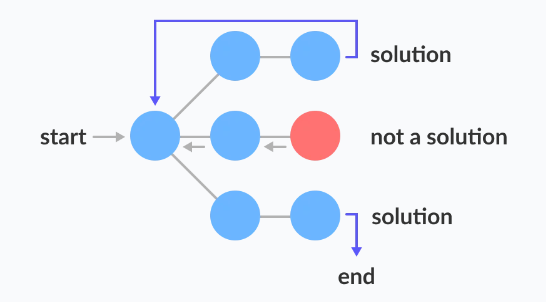
\includegraphics[width=0.8\textwidth]{Anh/mota_back_tracking}
	\caption{Mô tả thuật toán quay lui}
\end{figure}
Từ những đặc điểm chính ở trên ta có mã giả (pseudocode) của thuật toán như sau:
\begin{figure}[H]
	\centering
	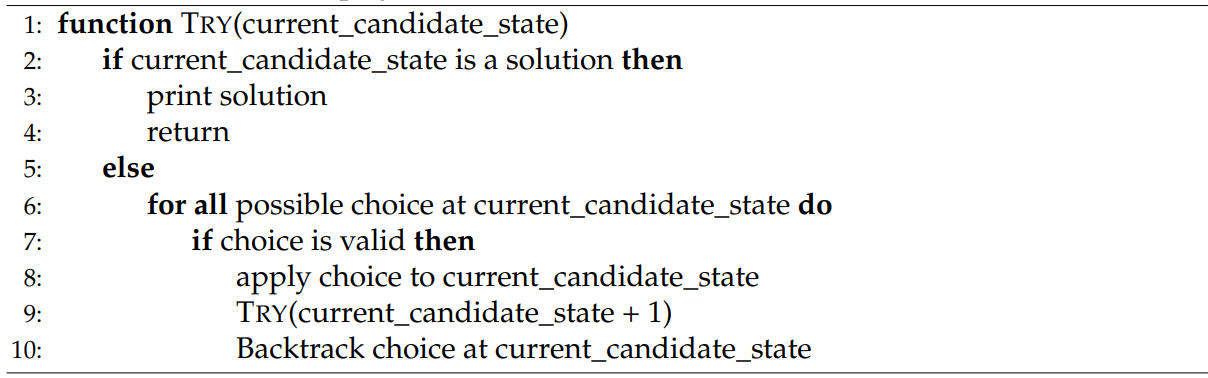
\includegraphics[width=\textwidth]{Anh/backtrack_pseudocode}
	%\caption{Mã giả thuật toán quay lui}
\end{figure}
Thuật toán xuất phát từ một trạng thái ứng cử viên cho lời giải (current\_candidate\_state), sau đó ta kiểm tra trạng thái có phải một lời giải hay không. Nếu không, với từng trạng thái có thể từ current\_candidate\_state ta chuyển sang trạng thái tiếp theo. Sau khi duyệt xong trạng thái tiếp theo của current\_candidate\_state, ta backtrack lại trạng thái ban đầu và duyệt tiếp trạng thái tiếp theo khác.
\subsection{Phương pháp thực hiện}
Để tìm lời giải tối ưu cho bài toán VRPTW đang xét, ta liệt kê tất cả các khả năng của bài toán và so sánh giá trị hàm mục tiêu của các khả năng với nhau. Gọi $(c,v)$ là một ứng cử viên với:
\begin{itemize}
	\item $c\in C$. Trong đó, $C$ là tập các khách hàng
	\item $v\in V$. Trong đó, $V$ là tập các xe
\end{itemize}
\begin{thuattoan}
	[Backtracking for VRPTW].
	\begin{itemize}
		\item \textbf{Bước khởi tạo:} Khai báo biến tối ưu $\min = +\infty$
		\item \textbf{Bước 1:} Chọn lần lượt từng ứng cử viên $(c,v)$ theo thứ tự $c, v$ đánh số tăng dần, chỉ chọn những ứng cử viên chưa được thăm
		\item \textbf{Bước 2:} Kiểm tra trạng thái của ứng cử viên hiện tại. Với một khả năng tìm được, ta so sánh với giá trị tối ưu hiện tại $\min$
		\item \textbf{Bước 3:} Nếu chưa tìm được khả năng thỏa mãn hoặc đã duyệt xong một khả năng thỏa mãn, ta quay lại bước 1 để tìm ứng cử viên tiếp theo
	\end{itemize}
\end{thuattoan}
\subsection{Kết quả}
Thuật toán duyệt qua toàn bộ không gian bài toán. Mỗi khách hàng có $\abs{V}$ lựa chọn nên độ phúc tạp $O\ngoacto{\abs{V}^n}$\\
Do vậy thuật toán chỉ có thể chạy với những test case rất nhỏ. 
\newpage\section{Thuật toán đơn hình (Simplex Algorithm)}
\subsection{Khái quát thuật toán}
Phương pháp đơn hình giải quy hoạch tuyến tính do G.B.Danzig đề xuất vào năm 1947. Mặc dù, về mặt lý thuyết, thuật toán đơn hình có độ phức tạp mũ và cho đến nay, đã có nhiều thuật toán với độ phức tạp đa thức để giải quy hoạch tuyến tính như thuật toán elipsoid của Khachiyan (1974), thuật toán điểm trong của Karmarkar (1984), nhưng trong thực tế đơn hình vẫn là phương pháp được sử dụng nhiều nhất trong việc giải bài toán quy hoạch tuyến tính. Theo báo SIAM (5/2000) thuật toán đơn hình được đánh giá là một trong 10 thuật toán có ảnh hưởng nhất trong sự phát triển và ứng dụng của khoa học kỹ thuật trong thế kỷ 20.
\subsection{Cơ sở lý thuyết}
\subsubsection{Bài toán quy hoạch tuyến tính}
\begin{dnghia}
	Xét bài toán QHTT dạng \kniem{chính tắc (standard form)}:
	\begin{align}
		\min\quad &f(x) = \tichvohuong{c}{x} \\
		s.t:\quad &A x = b\notag\\
		&x \ge 0\notag
	\end{align}
	\begin{itemize}
		\item $f(x)$ là \kniem{hàm mục tiêu (objective function)}
		\item $x = \vectordong{x}\in\mathbb{R}^n$ là biến
		\item $c = \vectordong{c}$ là \kniem{vector hệ số} của hàm mục tiêu
		\item $D = \taphop{x\in\mathbb{R}^n \mid Ax = b, x\ge 0}$ là \kniem{tập nghiệm chấp nhận được} và:
		\begin{itemize}
			\item $D$ là tập lồi đa diện
			\item $b = \left(b_1, b_2, \ldots, b_m\right)^T \ge 0$ và 
			\item $A$ là ma trận cấp $m\times n$ có $rank A = m$ với các cột $A_1, A_2, \ldots, A_n$
		\end{itemize}
		\item \kniem{Nghiệm tối ưu} $x^*$ là nghiệm thỏa mãn $f\ngoacto{x^*} \le f(x), \forall x\in D$
		\item \kniem{Phương án cực biên - PACB} là phương án thỏa mãn chặt $n$ ràng buộc độc lập tuyến tính
		\begin{itemize}
			\item \kniem{PACB không suy biến} thỏa mãn chặt đúng $n$ ràng buộc
			\item \kniem{PACB suy biến} thỏa mãn chặt nhiều hơn $n$ ràng buộc
		\end{itemize}
	\end{itemize}
\end{dnghia}
\begin{chuy}
	"Nghiệm" hay "phương án" là hai khái niệm như nhau
\end{chuy}

\subsubsection{Phương án cực biên}
\begin{chuy}
	Ta chỉ xét bài toán QHTT có phương án cực biên không suy biến
\end{chuy}
\begin{dly}
	Phương án chấp nhận được $x^0\in D$ là phương án cực biên khi và chỉ khi các vector cột $\taphop{A_j \mid j \in J(x^0)}$ độc lập tuyến tính
\end{dly}
\begin{cm}
	Không mất tính tổng quát, ta xét $J(x^0) = \taphop{1,\ldots,k}$, tức là: 
	$$x^0 = \ngoacto{x^0_1, x^0_2, \ldots, x^0_k, 0, \ldots, 0}^T\text{ với } x^0_j > 0, j = \overline{1,k}$$
	Với $\forall x^0 \in D$ là phương án chấp nhận được ta có:
	\begin{equation} \label{eq:1}
		\tonglanluot{j=1}{k} x^0_j A_j = b
	\end{equation}
	\kniem{Chiều thuận:} Giả sử $A_1, A_2, \ldots, A_k$ phụ thuộc tuyến tính, khi đó tồn tại bộ số thực $d_1, d_2, \ldots, d_k$ không đồng thời bằng $0$ thỏa mãn:
	\begin{equation}
		\tonglanluot{j=1}{k} d_jA_j = 0
	\end{equation}
	Kết hợp với $(2)$ ta được: 
	\begin{equation}
		\tonglanluot{j=1}{k} \ngoacto{x^0_j \pm td_j}A_j = b\quad, \forall t\in \mathbb{R}^+
	\end{equation}
	Dễ thấy chỉ cần chọn $t$ đủ nhỏ ta hoàn toàn có thể có được $y, z\in D$ và $y \neq z$ thỏa mãn:
	\begin{equation}
		x = \dfrac{1}{2}. y +\dfrac{1}{2}. z
	\end{equation}
	là một tổ hợp lồi chặt của $x^0$, điều này mâu thuẫn do $x^0$ là phương án cực biên\\
	\kniem{Chiều đảo:} Giả sử $x^0$ không phải phương án cực biên, khi đó:
	\begin{equation}
		\exists\, y, z\in D, y\neq z: x^0 = \lambda y +(1-\lambda) z \quad, \lambda\in\khoang{0}{1}
	\end{equation}
	Dễ thấy rằng $y, z$ đều thỏa mãn $(2)$ và $y\neq z$ nên $A_1, A_2, \ldots, A_k$ phụ thuộc tuyến tính, mâu thuẫn với giả thiết độc lập tuyến tính đã cho 
	%Nhận thấy rằng nếu $x^0$ là phương án cực biên thì $x^0$ không thể biểu diễn bằng tổ hợp lồi chặt của hai điểm phân biệt bất kì nào thuộc $D$.\\ Điều đó đồng nghĩa rằng $(x^0_1, x^0_2, \ldots, x^0_k)$ là bộ số duy nhất để biểu diễn $b$ thông qua các vector cột $A_1, A_2, \ldots, A_k$, tức là $A_1, A_2, \ldots, A_k$ độc lập tuyến tính 
\end{cm}
\begin{nx}
	Từ trên ta nhận thấy rằng, mỗi phương án cực biên sẽ tương ứng với một và chỉ một bộ vector cột $A_1, A_2, \ldots, A_k$ độc lập tuyến tính
\end{nx}
\begin{hqua}
	Số thành phần dương trong mỗi phương án cực biên của bài toán QHTT chính tắc không vượt quá $m$
\end{hqua}
\begin{cm}
	Do ta mặc định ma trận $A$ cấp $m\times n$ và $rank A = m$ nên số vector cột độc lập tuyến tính (hay nói cách khác là số phương án cực biên) không thể vượt quá $m$ 
\end{cm}
\begin{hqua}
	Số phương án cực biên của bài toán QHTT chính tắc là hữu hạn
\end{hqua}
\begin{cm}
	Từ định lý trên ta có mỗi phương án cực biên tương ứng với một bộ $k\le m$ vector độc lập tuyến tính của $A$. Do ma trận có $n$ cột nên số bộ gồm $k$ vector có thể chọn là $C^k_n$. Vậy nên, tổng số phương án cực biên không thế vượt quá $\tonglanluot{k=0}{n}C^k_n = 2^n$
\end{cm}
\begin{nx}
	Đây là đặc điểm quan trọng để chi ra thuật toán đơn hình là hữu hạn và có độ phức tạp mũ. Ngoài ra, kết hợp với định nghĩa của phương án cực biên, ta có:
	\begin{itemize}
		\item $\abs{J(x^0)} = m$ khi $x^0$ là phương án cực biên không suy biến
		\item $\abs{J(x^0)} < m$ khi $x^0$ là phương án cực biên suy biến
	\end{itemize}
\end{nx}
\subsubsection{Điều kiện tối ưu}
\begin{dnghia}
	Một bộ gồm $m$ vector độc lập tuyến tính $B = \taphop{A_{j1}, A_{j2}, \ldots, A_{jm}}$ của ma trận $A$ cấp $m\times n$ có $rank A = m$ được gọi một \kniem{cơ sở} của ma trận $A$
\end{dnghia}
Giả sử ta biết trước phương án cực biên $x^0$, khi đó $\taphop{A_j \mid j\in J(x^0)}$ là cơ sở của ma trận $A$. Vậy nên với mỗi vector cột $A_k, k\in\taphop{1,2,\ldots,n}$ được biểu diễn dưới dạng
\begin{equation}
	A_k = \tonglanluot{j\in J\ngoacto{x^0}}{} z_{jk}A_j
\end{equation} với bộ số thực $z_{jk}, j\in J\ngoacto{x^0}$ được xác định duy nhất\\
Chú ý rằng $\forall\, y\in D$ ta có: $b = \tonglanluot{j = 1}{n} A_jy_j= \tong{j\in J(x^0)} A_jx^0_j$. Khi đó:
\begin{align*}
	\tong{j\in J(x^0)} A_j\ngoacto{y_j - x^0_j} &= -\tong{k\notin J(x^0)} A_k.y_k\\
	&= -\tong{k\notin J(x^0)} \ngoacto{\tonglanluot{j\in J\ngoacto{x^0}}{} z_{jk}A_j}.y_k\quad\text{ (theo (7))}\\
	&= -\tong{j\in J(x^0)} A_j\ngoacto{\tong{k\notin J(x^0)} z_{jk} y_k}
\end{align*}
Khi đó ta có \begin{equation}
	y_j - x^0_j = -\tong{k\notin J(x^0)} z_{jk} y_k
\end{equation}
Từ trên ta có:
\begin{align*}
	f(y) - f(x^0) &= \tong{k\notin J(x^0)} c_ky_k - \tong{j\in J(x^0)} c_j\ngoacto{y_j - x^0_j}\\
	&= \tong{k\notin J(x^0)} c_ky_k + \tong{j\in J(x^0)} c_j\ngoacto{-\tong{k\notin J(x^0)} z_{jk} y_k}\\
	&= \tong{k\notin J(x^0)} c_ky_k - \tong{k\notin J(x^0)} \ngoacto{\tong{j\in J(x^0)} z_{jk}c_j} y_k \\
	&= \tong{k\notin J(x^0)} \ngoacto{c_k -\tong{j\in J(x^0)} z_{jk}c_j} y_k \\
	&= -\tong{k\notin J(x^0)} \Delta_ky_k
\end{align*}
Từ đó, ta có định nghĩa sau:
\begin{dnghia}
	\kniem{Ước lượng} của biến $x_k$ là: $$\Delta_k = \tonglanluot{j\in J\ngoacto{x^0}}{} z_{jk}c_j - c_k,\quad k\in\taphop{1,2,\ldots,n}$$
\end{dnghia}
Từ định nghĩa trên, ta có:
\begin{dly}[Kiểm tra phương án cực biên]
	Cho $x^0$ là phương án cực biên:
	\begin{itemize}
		\item Nếu $\forall k\notin J(x^0)$ thỏa mãn $\Delta_k \le 0$ thì $x^0$ là phương án tối ưu
		\item Nếu $\begin{cases}
			\exists\, k\notin J(x^0)\\
			\forall\, j\in J(x^0)
		\end{cases}$ thỏa mãn $\Delta_k > 0 \text{ và } z_{jk} \le 0$ thì hàm mục tiêu giảm vô hạn trên tập chấp nhận được và bài toán không có lời giải
		\item Nếu $\begin{cases}
			\exists\, k\notin J(x^0)\\
			\exists\, j\in J(x^0)
		\end{cases}$ thỏa mãn $\Delta_k > 0 \text{ và } z_{jk} > 0$ thì ta có thể chuyển tới phương án cực biên $x^1$ tốt hơn $x^0$
	\end{itemize}
\end{dly}
\begin{cm}
	Từ $(7)$ ta viết lại:
	\begin{equation}
		b = \tong{j\in J(x^0)} A_jx^0_j = \tong{j\in J(x^0)} A_j\ngoacto{x^0_j - \theta z_{jk}} + \theta A_k\quad, \forall \theta\in\mathbb{R}^+
	\end{equation}
	Vì vậy, nếu đảm bảo được điều kiện
	\begin{equation}
		x^0_j - \theta z_{jk} > 0 \quad, \forall j\in J(x^0)
	\end{equation}
	Ta được phép xét các điểm $y=\vectordong{y}\in D$ có tọa độ xác định bởi:
	\begin{equation*}
		y_j = \left\{\begin{array}{cl}
			x^0_j - \theta z_{jk} &\quad, \forall j\in J(x^0)\\
			0 &\quad, \forall j\notin J(x^0) \text{ và } j\neq k\\
			\theta &\quad, j=k
		\end{array}\right.
	\end{equation*}
	Dễ thấy $y = x^0 + \theta z^k$. Trong đó vector $z^k$ cố định được xác định bởi:
	\begin{equation*}
		z^k_j = \left\{\begin{array}{cl}
			-z_{jk} &\quad, \forall\, j\in J(x^0)\\
			0 &\quad, \forall\, j\notin J(x^0) \text{ và } j\neq k\\
			1 &\quad, j=k
		\end{array}\right.
	\end{equation*}
	Điều đó có nghĩa rằng $y$ là một điểm nằm trên tia xuất phát từ $x^0$ theo hướng của vector $z^k$\\
	Khi đó, theo ... ta có:
	\begin{equation}
		f(y) - f(x^0) = -\tong{k\notin J(x^0)} \Delta_k y_k = -\theta\Delta_k
	\end{equation}
	Từ đây, dễ thấy nếu $\exists\, \Delta_k > 0$ và $z_{jk} \le 0, \forall\, j\in J(x^0)$ thì khi ta cho: $$\theta \rightarrow +\infty \Rightarrow f(y) \rightarrow -\infty$$
	Lúc này hàm mục tiêu giảm vô hạn và bài toán không có lời giải\\
	Ngược lại, nếu $\exists\, j\in J(x^0)$ sao cho $z_{jk} > 0$. Khi này, hoàn toàn có thể tìm được phương án có thể làm giảm hàm mục tiêu. Tuy nhiên, phương án được chọn phải là phương án cực biên. Để đảm bảo điều kiện $(10)$ của phương án chấp nhận được, ta chọn:
	\begin{equation*}
		x^1_j = \left\{\begin{array}{cl}
			x^0_j - \theta_0 z_{jk} &\quad, \forall j\in J(x^0)\\
			0 &\quad, \forall j\notin J(x^0) \text{ và } j\neq k\\
			\theta_0 &\quad, j=k
		\end{array}\right.
	\end{equation*}
	Trong đó:
	\begin{equation}
		\theta_0 = \min\taphop{\dfrac{x_j^0}{z_{jk}}\mid z_{jk} > 0, j\in J(x^0)} = \dfrac{x_r^0}{z_{rk}}\text{ với } r \in J(x^0)
	\end{equation}
	Khi đó ta xét $J(x^1) = \ngoacto{J(x^0) \setminus \taphop{r}} \cup \taphop{k}$ có $\abs{J(x^1)} = \abs{J(x^0)} = m$ và kiểm tra được hệ $\taphop{A_j\mid j\in J(x^1)}$ độc lập tuyến tính, tức $x^1$ là một PACB với bộ chỉ số cơ sở $J(x^1)$
\end{cm}

\begin{tc}
	[Quy tắc] Chọn chỉ số vector đưa vào và ra khỏi cơ sở ban đầu:
	\begin{itemize}
		\item Chọn $s$ là chỉ số thỏa mãn $$\Delta_s = \max\taphop{\Delta_k \mid \Delta_k > 0}$$ là \kniem{chỉ số của vector đưa vào cơ sở mới} có ước lượng lớn nhất để giảm giá trị hàm mục tiêu nhiều nhất. 
		\item Chọn $r$ là chỉ số xác định bởi $$\theta_0 = \min\taphop{\dfrac{x^0_j}{z_{js}} \mid z_js > 0, j\in J(x^0)} = \dfrac{x^0_r}{z_{rs}}\text{ với } r\in J(x^0)$$
		\item Đưa $A_s$ vào và $A_r$ ra khỏi cơ sở và nhận được PACB mới $x^1 = \ngoacto{x^1_1, x^1_2, \ldots, x^1_n}^T$ với $$x^1_j = \begin{cases}
			x^0_j -\dfrac{x^0_r}{z_{rs}}z_{js} &, \forall j\in \ngoacto{J(x^0)\setminus\taphop{r}}\\
			0 &, \forall j \notin \ngoacto{J(x^0)\setminus\taphop{r}\cup\taphop{s}}\\
			\dfrac{x^0_r}{z_{rs}} &, j = s
		\end{cases}$$
	\end{itemize}
\end{tc}
Từ quy tắc vừa đề cập, ta đến với phần tiếp theo.
\subsection{Phương pháp thực hiện}
\subsubsection{Thuật toán đơn hình giải LP chính tắc}
\begin{thuattoan}[Đơn hình - Simplex Algorithm].
	\begin{itemize}
		\item \textbf{Bước khởi tạo:} Xuất phát từ phương án cực biên $x^0$ và cơ sở $\taphop{A_j \mid j\in J\ngoacto{x^0}}$
		\item \textbf{Bước 1:} Tính giá trị hàm mục tiêu: $$f\ngoacto{x^0} = \tonglanluot{j\in J\ngoacto{x^0}}{} c_jx^0_j$$
		\item \textbf{Bước 2:} Với mỗi $k \notin J\ngoacto{x^0}$, xác định các số $z_{jk}$ bằng việc giải hệ $$\tonglanluot{j\in J\ngoacto{x^0}}{} z_{jk} A_j = A_k$$ và tính các ước lượng $$\Delta_k = \tonglanluot{j\in J\ngoacto{x^0}}{} z_{jk} c_j -c_k$$
		\item \textbf{Bước 3: (Kiểm tra điều kiện tối ưu)} Xét $\Delta_k$:
		\begin{itemize}
			\item Nếu $\Delta_k \le 0, \forall k\notin J\ngoacto{x^0}$ thì dừng thuật toán và $x^0$ là nghiệm tối ưu
			\item Nếu ngược lại thì sang bước 4
		\end{itemize}
		\item \textbf{Bước 4: (Kiểm tra không có lời giải)}
		\begin{itemize}
			\item Nếu $\exists k \in J\ngoacto{x^0}$ sao cho $\Delta_k > 0$ và $z_{jk} \le 0, \forall j\in J\ngoacto{x^0}$ thì dừng thuật toán và bài toán không có nghiệm tối ưu
			\item Nếu ngược lại thì chuyển sang bước 5
		\end{itemize}
		\item \textbf{Bước 5: (Xây dựng phương án cực biên mới)}
		\begin{itemize}
			\item Tìm vector $A_s$ để đưa vào cơ sở mới với $s$ được chọn có $$\Delta_s = \max\taphop{\Delta_k \mid \Delta_k > 0}$$
			\item Tìm vector $A_r$ để đưa ra khỏi cơ sở cũ với $r$ được chọn có $$\theta_0 = \min\taphop{\dfrac{x^0_j}{z_{js}} \mid z_{js} > 0} = \dfrac{x^0_r}{z_{rs}}$$
			\item Xây dựng phương án cực biên mới theo công thức đổi cơ sở và cơ sở mới là $$x^1_j = \begin{cases}
			x^0_j -\dfrac{x^0_r}{z_{rs}}z_{js} &, \forall j\in \ngoacto{J(x^0)\setminus\taphop{r}}\\
			0 &, \forall j \notin \ngoacto{J(x^0)\setminus\taphop{r}\cup\taphop{s}}\\
			\dfrac{x^0_r}{z_{rs}} &, j = s
		\end{cases}$$
			\item Đặt $x^0 := x^1$ và quay lại bước 1
		\end{itemize}
	\end{itemize}
\end{thuattoan}
% \paragraph{Công thức đổi cơ sở}
% Ta có tập chỉ số cơ sở mới $x^1$ kề với $x^0$ là:
% \begin{equation}
% 	J(x^1) = \ngoacto{J(x^0) \setminus \taphop{r}} \cup \taphop{s}
% \end{equation}
% Khi đó ta có: 
% \begin{equation}
% 	A_s = \tong{j\in J(x^0)} z_jsA_j \Rightarrow A_r = \dfrac{1}{z_{rs}}\ngoacto{A_s - \tong{j\in J(x^0)\setminus\taphop{r}} z_{js}A_j} 
% \end{equation}
% Với mỗi $k\in\taphop{1, 2, \ldots, n}$ ta có:
% \begin{align*}
% 	A_k = \tong{j\in J(x^0)} z_{jk} A_j &= \tong{j\in J(x^0)\setminus\taphop{r}} z_{jk}A_j + z_{rk}A_r\\
% 	&= \tong{j\in J(x^0)\setminus\taphop{r}} z_{jk}A_j + \dfrac{z_{rk}}{z_{rs}} \ngoacto{A_s - \tong{j\in J(x^0)\setminus\taphop{r}} z_{js}A_j}\\
% 	&= \tong{j\in J(x^0)\setminus\taphop{r}} \ngoacto{z_{jk} - \dfrac{z_{rk}}{z_{rs}} z_{js}} A_j + \dfrac{z_{rk}}{z_{rs}}A_s = \tong{j \in J(s^1)} z^1_{jk} A_j
% \end{align*}
% Từ đây ta có công thức biểu diễn $A_k$ qua cơ sở mới:
% \begin{equation*}
% 	z^1_{jk} = \left\{\begin{array}{cl}
% 		z_{jk} - \dfrac{z_{rk}}{z_{rs}} z_{js} &\quad, j\in J(x^1)\setminus\taphop{s}\\
% 		\dfrac{z_{rk}}{z_{rs}} &\quad, j=s
% 	\end{array}\right.
% \end{equation*}
% Các ước lượng mới có thể xác định bằng công thức 
% \begin{equation}
% 	\Delta_k^1 = \tong{j\in J(x^1)}z^1_{jk}c_j - c_k
% \end{equation}
% \newpage Hoặc ta có thể tính qua công thức sau:
% \begin{equation}
% 	\Delta_k^1 = \Delta_k - \dfrac{z_{rk}}{z_{rs}}\Delta_s
% \end{equation}

\subsubsection{Thuật toán đơn hình dạng bảng}
\paragraph{Bảng đơn hình}
\begin{longtblr}[
	caption={Minh họa bảng đơn hình},
	label={tab:simplex}
	]{
		colspec = {||c|c|c|c c c c c| c||},
		%width = ,
		rowhead = 1, % Đặt chiều rộng của bảng
		rowsep = 5pt, % Đặt khoảng cách giữa các dòng
	}
	\hline
	\SetCell[r=2]{c} Hệ số $C_B$ & \SetCell[r=2]{c} Cơ sở $B$ & \SetCell[r=2]{c} Phương án & $c_1$			& $\ldots$ 	& $c_k$ 		& $\ldots$ 	& $c_n$ 		& \SetCell[r=2]{c} $\theta$		\\
	&          						&          							& $A_1$			& $\ldots$ 	& $A_k$ 		& $\ldots$ 	& $A_n$ 		&								\\\hline
	$c_{j_1}$ 	& $A_{j_1}$ & $x^0_{j_1}$ 	& $z_{j_11}$ 	& $\ldots$ 	& $z_{j_1k}$ 	& $\ldots$ 	& $z_{j_1n}$ 	& $\theta_{j_1}$\\
	$\vdots$ 	& $\vdots$ 	& $\vdots$ 		& $\vdots$ 		& 			& $\vdots$ 		& 			& $\vdots$ 		& $\vdots$ 		\\
	$c_{j}$ 	& $A_{j}$ 	& $x^0_{j}$ 	& $z_{j1}$ 		& $\ldots$ 	& $z_{jk}$ 		& $\ldots$ 	& $z_{jn}$ 		& $\theta_{j}$	\\
	$\vdots$ 	& $\vdots$ 	& $\vdots$ 		& $\vdots$ 		& 			& $\vdots$ 		& 			& $\vdots$ 		& $\vdots$ 		\\
	$c_{j_m}$ 	& $A_{j_m}$ & $x^0_{j_m}$ 	& $z_{j_m1}$ 	& $\ldots$ 	& $z_{j_mk}$ 	& $\ldots$ 	& $z_{j_mn}$ 	& $\theta_{j_m}$\\	\hline
	&			& $f(x^0)$ 		& $\Delta_1$ 	& $\ldots$ 	& $\Delta_2$ 	& $\ldots$ 	& $\Delta_n$ 	& 				\\	\hline
\end{longtblr}
Bảng đơn hình gồm $n+4$ cột
\begin{itemize}
	\item Cột 1: (Hệ số $C_B$) Ghi giá trị hệ số hàm mục tiêu ứng với các biến cơ sở
	\item Cột 2: (Cơ số $B$) Ghi tên các vector cơ sở.
	\item Cột 3: (Phương án cực biên) Ghi giá trị của các biến cơ sở của phương án cực biên đang xét
	\item $n$ cột tiếp theo. Cột thứ $3+k$ ứng với tên vector $A_k$. Phía trên tên mỗi cột $A_k$ ghi giá trị hệ số của hàm mục tiêu $c_k$ tương ứng
	\item Cột cuối cùng. Dành để ghi tỷ số $\theta_j, j\in J_B$
	\item Dòng cuối cùng. Tại vị trí dưới cột $3$, ghi giá trị hàm mục tiêu tại phương án cực biên đang xét
	\begin{equation}
		f(x^0) = \tong{j\in J_B} x_jx^0_j
	\end{equation}
	Tại vị trí dưới cột ứng với vector $A_k$ ghi các ước lượng $$\Delta_k = \tong{j\in J_B} z_{jk}c_j - c_k$$
	Ta có $\Delta_j = 0, \forall\, j\in J_B$
\end{itemize}
\begin{thuattoan}[Đơn hình dạng bảng].
	\begin{itemize}
		\item \textbf{Bước khởi tạo:} Xây dựng bảng đơn hình xuất phát tương ứng với phương án cực biển $x^0$
		\item \textbf{Bước 1: (Kiểm tra điều kiện tối ưu)} Xét dòng cuối của bảng:
		\begin{itemize}
			\item Nếu $\Delta_k \le 0, \forall k = 1,\ldots, n$ thì dừng thuật toán và nghiệm tối ưu là phương án cực biên của bảng này
			\item Nếu ngược lại, chuyển sang bước 2
		\end{itemize}
		\item \textbf{Bước 2: (Kiểm tra bài toán không có lời giải)}
		\begin{itemize}
			\item Nếu $\begin{cases}
				\exists\, k\in J_B\\
				\forall\, j\in J_B
			\end{cases}$ sao cho $\Delta_k > 0$ và $z_{jk} \le 0$ thì dừng thuật toán và không có lời giải
		\end{itemize}
		\item \textbf{Bước 3:} Thực hiện:
		\begin{itemize}
			\item Tìm cột quay: Xác định $A_s$ để đưa vào cơ sở mới được gọi là \kniem{cột quay}
			\item Tìm dòng quay: Tính các $\theta_j, j\in J_B$ như sau: $$\theta_j = \begin{cases}
				\dfrac{x_j}{z_{js}} &\text{, nếu } z_{js} > 0, j\in J_B\\
				+\infty &\text{, nếu } z_{js} \le 0, j\in J_B
			\end{cases}$$ và xác định $\theta_r = \min\taphop{\theta_j \mid j\in J_B}$\\
			Dòng $r$ được gọi là \kniem{dòng quay} và giao của dòng quay và cột quay là \kniem{phần tử chính của phép quay}. Các phần tử $z_{js}\ngoacto{j\neq r}$ được gọi là \kniem{phần tử quay}
		\end{itemize}
		\item \textbf{Bước 4: (Chuyển bảng mới tương ứng với phương án cực biên mới)} Thực hiện:
		\begin{itemize}
			\item Trong cột hệ số $C_B$ và cột cơ sở thay các giá trị và ký hiệu của $r$ thành $s$
			\item Chia các phần tử của dòng quay cho phần tử chính ta được dòng mới gọi là \kniem{dòng chính}: $$\textbf{Dòng chính (mới)} := \dfrac{\textbf{Dòng quay (cũ)}}{\textbf{Phần tử chính}}$$
			\item Biến đổi mỗi dòng còn lại theo quy tắc: $$\textbf{Dòng mới} := \textbf{Dòng cũ tương ứng} - \textbf{Dòng chính} \times \textbf{Phần tử quay tương ứng}$$ Ta được số $0$ ở mọi vị trí còn lại trong cột quay cũ
			\item Quay lại bước 1 với bảng mới
		\end{itemize}
	\end{itemize}
\end{thuattoan}
\subsubsection{Thuật toán đơn hình hai pha}
\begin{thuattoan}[Đơn hình hai pha].
	\begin{itemize}
		\item \textbf{Pha 1: (Tìm phương án cực biên xuất phát cho thuật toán đơn hình giải QHTT chính tắc)}. Xây dựng bài toán phụ: ta cộng thêm biến giả vào những phương trình cần thiết để tạo ra ma trận $m$ cột là các vector đơn vị khác nhau. Giải bài toán QHTT chính tắc phụ \begin{equation}
			\min\taphop{g(x, u) \mid Ax + u = b, \ngoacto{x, u} \ge 0}
		\end{equation} nhận được phương án cực biên tối ưu $\ngoacto{x^0, u^0}$
		\begin{itemize}
			\item Nếu $g(x^0, u^0) > 0$ thì $D = \varnothing$, dừng thuật toán
			\item Nếu ngược lại ($x^0$ là phương án cực biên của bài toán QHTT chính tắc). Chuyển sang pha 2
		\end{itemize}
		\item \textbf{Pha 2:} Giải bài toán QHTT chính tắc đang xét bằng phương pháp đơn hình xuất phát từ phương án cực biên $x^0$ và chú ý rằng bảng đơn hình đầu tiên của Pha 2 là bảng đơn hình cuối cùng ở Pha 1 nhưng với một số sửa đổi sau:
		\begin{itemize}
			\item Xóa tất cả các cột tương ứng với các biến giả
			\item Thay cột $C_B$ bởi hệ số mục tiêu cơ sở tương ứng với bài toán gốc
			\item Thay các hệ số mục tiêu của bài toán ở dòng 1 bằng hệ số mục tiêu của bài toán gốc
			\item Nếu trong cơ sở tương ứng với phương án tối ưu của bài toán QHTT chính tắc không có vector giả thì cơ sở ứng với phương án này cũng chính là cơ sở tương ứng với $x^0$. Để có bảng đơn hình xuất phát cho bài toán ban đầu, ta chỉ cần tính lại giá trị hàm mục tiêu tại $x^0$ và tính lại các ước lượng theo công thức $$f(x^0) = \tongchisocoso c_jx_j^0 \text{ và } \Delta_k = \tongchisocoso z_{jk}c_j - c_k$$
			\item Nếu trong cơ sở của phương án cực biên tối ưu của bài toán QHTT chính tắc phụ có ít nhất một vector giả thì ta nhận được một phương án cực biên suy biến của bài toán ban đầu, tức là $J(x^0) = \taphop{j\in\taphop{1,\ldots,n} \mid x_j^0 > 0} < m$. Khi đó, để đẩy hết biến giả ra khỏi cơ sở ta thực hiện thêm một vài vước lặp đơn hình nữa như sau: Chọn cột quay là cột ứng với vector phi cơ sở $A_k$ với $k\le n$ (tức là $A_k$ không phải vector giả) mà nó có phần tử khác $0$ ở dòng tương ứng với vector giả và dòng này được chọn là dòng quay. Chú ý, phần tử chính lúc này có thể dương hoặc âm (khác $0$). Do giả thiết $rank A = m$ nên nếu có biến giả trong cơ sở thì chắc chắn sẽ tìm được cột quay như thế. Sau khi bổ sung vector để nhận được cơ sở $B = \taphop{A_j, j\in J}$ với $J \supset J(x^0)$, ta bỏ các cột tương ứng với biến giả rồi tiếp thục thuật toán.
		\end{itemize}
	\end{itemize}
\end{thuattoan}
\subsection{Kết quả}
Theo hệ quả $2$, số đỉnh tối đa là $2^n$ nên trong trường hợp xấu nhất, độ phức tạp của thuật toán là $O\ngoacto{2^n}$. Tuy nhiên, trong thực tế thuật toán có thể tìm ra phương án tối ưu mà không cần duyệt qua tất cả các đỉnh của đa diện nên độ phức tạp trung bình có thể giảm đi đáng kể so với độ phức tạp hàm số mũ ở trên.\\
Ta thấy độ phức tạp của bài toán trên là quá lớn để áp dụng vào các bài toán thực tế. Vì vậy, ta cần các thuật toán cải thiện hơn về mặt tốc độ.

\newpage\section{ Thuật toán Gomory}
\subsection{Khái quát}
Quy hoạch nguyên là mô hình toán học của nhiều bài toán trong thực tế. Ví dụ trong một số bài toán như bài toán vận tải sản lượng hàng yêu cầu các biến hàng hóa, thời gian là số nguyên hay các biến quyết định là một tập rời rạc. Một trong những phương pháp để giải quyết các bài toán quy hoạch nguyên là thuật toán Gomory.\\

Xét bài toán quy hoạch nguyên tuyến tính: 
\begin{align}
	\min\quad &\tonglanluot{j=1}{n} c_j x_j \\
	s.t\quad &\tonglanluot{j=1}{n} a_{ij} x_j = b_i, i=\overline{1,m}\\
	& x_j \ge 0, j = \overline{1,n}\\
	& x_j \in \mathbb{Z}, j = \overline{1, n_1} (n_1 \le n)
\end{align}
\begin{itemize}
	\item Nếu $n_1 = n$ thì bài toán được gọi là bài toán quy hoạch tuyến tính nguyên toàn phần
	\item Nếu $n_1 < n$ thì bài toán được gọi là bài toán quy hoạch tuyến tính nguyên bộ phận 
\end{itemize}

Với thuật toán Gomory, ta sẽ đi giải quyết bài toán QHTT nguyên toàn phần
\subsection{Cơ sở lý thuyết}
\subsubsection{Ý tưởng}
Ý tưởng của thuật toán Gomory là từ tập đa diện lồi của tập chấp nhận được, ta sẽ cắt đa diện đó sao cho không mất đi điểm nguyên nào của nó. Cũng như các đỉnh mới của đa diện đều là nguyên. \\
Từ ý tưởng đó, ta sẽ thêm các ràng buộc vào bài toán ban đầu để các đỉnh của đa diện lồi chấp nhận được đều là các điểm nguyên
\begin{figure} [H]
    \centering
    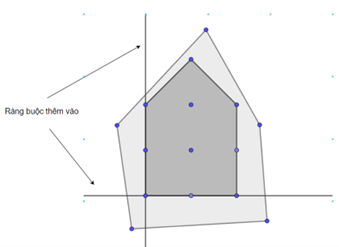
\includegraphics{Anh/mota_latcat}
    \caption{Minh họa cắt tập đa diện lồi}
    \label{fig:1}
\end{figure}
\subsubsection{Lát cắt đúng}
\begin{dnghia}
	Giả sử tập các điểm nguyên của một đa diện lồi $D = \taphop{ x\in \mathbb{Z}^n_+ \mid Ax \le b}$. Khi đó ta gọi ràng buộc $\alpha x \le \beta$ là \kniem{lát cắt đúng} của tập $D$ nếu: $$\alpha x \le b, \forall x\in D$$
\end{dnghia}
Nói cách khác, một ràng buộc được gọi là lát cắt đúng nếu nó không cắt đi bất cứ phương án nguyên nào của tập $D$

\begin{dly}
	Giả sử $\alpha x \le \beta$ là một lát cắt đúng của $D = \taphop{ x\in \mathbb{Z}^n_+ \mid Ax \le b}$. Khi đó, ta có:
	\begin{equation}
		\tonglanluot{i = 1}{n}\phannguyen{a_i} x_i \le \phannguyen{\beta}
	\end{equation}
	cũng là một lát cắt đúng của $D$. Với $\phannguyen{t} \in Z$ được gọi là phần nguyên của $t$
\end{dly}
\begin{cm}
	Do $\phannguyen{\alpha_i} \le \alpha_i$ và $x_i \ge 0$ nên ta có:
	$$\tonglanluot{i=1}{n} \phannguyen{a_i} x_i \le \tonglanluot{i=1}{n} a_i x_i \le \beta\,, \forall x\in D$$  
	Mặt khác vì $\tonglanluot{i=1}{n} \phannguyen{a_i} x_i \in \mathbb{Z}_+$ nên:
	$$\tonglanluot{i=1}{n} \phannguyen{a_i} x_i \le \phannguyen{\beta}, \forall x\in D$$
\end{cm}


\begin{dly}
	Giả sử rằng ràng buộc $\alpha x = \beta$ là một lát cắt đúng của $D$. Khi đó:
	\begin{equation}
		\tonglanluot{i=1}{n} \ngoacto{a_i - \phannguyen{a_i}}x_i \ge \beta - \phannguyen{\beta}
	\end{equation}
	tức là 
	\begin{equation*}
		\tonglanluot{i=1}{n}\taphop{a_i} x_i \ge \taphop{\beta}
	\end{equation*}
	cũng là một lát cắt đúng của $D$
\end{dly}
\begin{cm}
	Do $\alpha x = \beta$ là một lát cắt đúng của $D$ nên ta có:
	\begin{equation}
		\left\{
		\begin{array}{ccc}
			\tonglanluot{i = 1}{n} \alpha_i x_i &=& \beta \\
			\tonglanluot{i = 1}{n} \phannguyen{\alpha_i} x_i &\le& \phannguyen{\beta}
		\end{array}
		\right.\quad, \forall x\in D
	\end{equation}
	Trừ vế với vế ta có:
	\begin{equation}
		\tonglanluot{i=1}{n} \ngoacto{a_i - \phannguyen{a_i}} x_i \ge \beta - \phannguyen{\beta} \text{ Hay viết cách khác:} \tonglanluot{i=1}{n}\taphop{a_i} x_i \ge \taphop{\beta}\quad, \forall x\in D
	\end{equation}
	Ta có điều phải chứng minh
\end{cm}
\subsubsection{Tư tưởng phương pháp cắt của Danzig}
Ta ký hiệu $L^N$ là bài toán QHTT nguyên toàn phần, $L$ là bài toán QHTT.
\begin{enumerate}
	\item Việc giải $L^N$ là quá trình nhiều bước:
		\begin{itemize}
			\item Ở bước thứ $r$, ta giải bài toán QHTT phụ $\ngoacto{L_r},\, r=0,1,\ldots$ với $L_0 = L$
			\item Tập các điểm nguyên của đa diện lồi là như nhau: $$L^N_0 = L^N_1 = \ldots = L^N_r = \ldots$$\\
			Do đó nếu phương án tối ưu $X(L_r)$ của bài toán $L_r$ thỏa mãn điều kiện nguyên toàn phần thì nó cũng chính là phương án tối ưu $X(L^N)$ của bài toán xuất phát $L^N$ và quá trình kết thúc
			\item Nếu $X(L_r)$ không thỏa mãn điều kiện nguyên thì $X(L_r)\notin L_{r+1}$. Tức là nghiệm tối ưu của bài toán $L_r$ sẽ không thuộc đa diện lồi của bài toán $L_{r+1}$
		\end{itemize}
	\item Chuyển từ bước $r$ sang $r+1$ hay chuyển từ bài toán $L_r$ sang bài toán $L_{r+1}$ khi $X(L_r)$ không nguyên nhờ một lát cắt đúng $\alpha_r x\le \beta_r$
\end{enumerate}
\begin{nx}
	Như vậy bài toán được xem như có hai công đoạn: Nới lỏng ràng buộc nguyên của bài toán QHTT, chuyển từ bước này sang bước khác nhờ một lát cắt đúng.
\end{nx}
\begin{figure} [H]
    \centering
    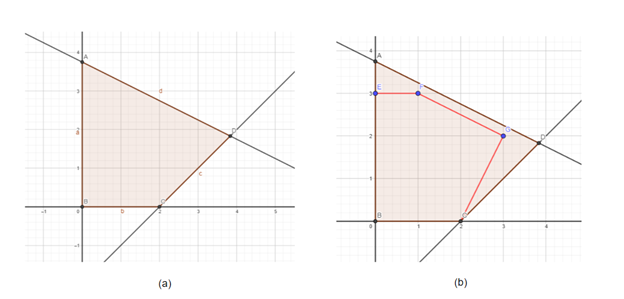
\includegraphics{Anh/mota_gomory}
    \caption{(a) tập chấp nhận được của bài toán gốc. (b) sau khi dùng Gomory cắt}
    \label{fig:2}
\end{figure}
\subsection{Phương pháp thực hiện}
Theo ý tưởng Danzig. Ta nới lỏng điều kiện nguyên, giải bài toán QHTT thu được nghiệm $x_0$, khi đó ta biểu diễn các biến cơ sở thông qua các biến phi cơ sở 
\begin{equation}
	x^0_{i0} = x^0_{i} + \tonglanluot{j \notin J(x^0)}{} z_{ji} x_j, i = 1,\ldots, n
\end{equation}
Ta có $a_k = \phannguyen{a_k} + \taphop{a_k}$. Khi đó (1) được viết lại dưới dạng
\begin{align}
	\phannguyen{x^0_{i0}} + \taphop{x^0_{i0}} &= x^0_{i} + \tonglanluot{j \notin J(x^0)}{} \ngoacto{\phannguyen{z_{ji}} + \taphop{z_{ji}}} x_j, i = 1,\ldots, n\notag\\
	-\phannguyen{x_{i0}^0} + x_i^0 + \tonglanluot{j\notin J(x^0)}{}\phannguyen{z_{ji}} x_j &= \taphop{x^0_{i0}} - \tonglanluot{j\notin J(x^0)}{}\taphop{z_{ji}} x_j
\end{align}
Để ý là $VT$ (12) phải nguyên, $VP$ của $12$ cũng phải là số nguyên nhỏ hơn $1$ (vì $\taphop{x^0_{i0}} < 1)\\
\Rightarrow $ VP của (12) luôn nhỏ hơn hoặc bằng $0$\\
Đặt $-x_k = VT(12) = -\phannguyen{x_{i0}^0} + x_i^0 + \tonglanluot{j\notin J(x^0)}{}\phannguyen{z_{ji}} x_j$, ta được $$\taphop{x_{i0}^0} - \tonglanluot{j\notin J(x^0)}{}\taphop{z_{ji}} x_j = -x_k$$
(với điều kiện $x_k$ nguyên và không âm)
\begin{equation}
	\Rightarrow -\tonglanluot{j\notin J(x^0)}{}\taphop{z_{ji}} x_j + x_k = -\taphop{x_{i0}^0}
\end{equation}
Theo mệnh đề 3.3 thì $(31)$ xác định một lát cắt đúng.

\begin{thuattoan}[Gomory].
	\begin{itemize}
		\item \textbf{Bước khởi tạo: } Giải bài toán quy hoạch tuyến tính không nguyên $$\min \langle c, x\rangle\quad v.d.k\quad x\in D$$ được nghiệm tối ưu $x^1$. Đặt $k := 1$ và $D_1 = D$
		\item \textbf{Bước lặp $k$}
		\begin{itemize}
			\item \textbf{Bước 1:} Nếu $x^k$ có các tọa độ nguyên thì chuyển sang Bước kết thúc
			\item \textbf{Bước 2:} Ngược lại $x^k$ có ít nhất một tọa độ không nguyên thì cần chọn ra một biến cơ sở có giá trị không nguyên để xây dựng ràng buộc bổ sung (lát cắt thứ $k$)
			$$-\tonglanluot{j\notin J(x^0)}{} \taphop{z_{ji}} x_j + x_k = -\taphop{x_{i0}^0}$$
			\item \textbf{Bước 3:} Giải bài toán thu được bằng phương pháp đơn hình 2 pha để tìm phương án tối ưu. Đặt $k:=k+1$ và chuyển về bước 1.
		\end{itemize}
		\item \textbf{Bước kết thúc:} Dừng và đưa ra kết quả kết thúc
	\end{itemize}
\end{thuattoan}
\subsection{Kết quả}
Với bộ dữ liệu bé $(n<10)$ thì thuật toán tính toán rất chậm. Để cắt ra được bao lồi các điểm nguyên thì phải thực hiện qua nhiều bước lặp. Do vậy cần kết hợp thêm một số thuật toán khác như nhánh cận để giảm khối lượng tính toán.
\newpage\section{ILP formulation}
\subsection{Nhắc lại bài toán và mục tiêu tối ưu}
Bài toán được phát biểu bởi đồ thị $G = (V, E)$, trong đó tập đỉnh $V$ là các khách hàng và kho chứa. Mỗi khách hàng sẽ có nhu cầu về số lượng hàng hóa khác nhau và chỉ mở cửa phục vụ trong thời gian nhất định $\ngoacvuong{T_a, T_b}$. Tập cạnh $E$ là mạng lưới đường đi giữa các khách hàng và kho. Trong bài toán này, khoảng cách giữa hai điểm được xem như thời gian di chuyển giữa hai điểm đó (ta xem thời gian và quãng đường đi là tuyến tính). Phục vụ các khách hàng là $V$ xe, mỗi xe có sức chứa cố định và như nhau. Các xe sẽ xuất phát và quay lại kho chứa. Không nhất thiết phải sử dụng hết tất cả các xe và mỗi khách hàng chỉ được phục vụ bởi một xe duy nhất. Khi xe đến phục vụ khách hàng thứ $i$ sẽ mất thười gian phục vụ $T_{si}$ và các xe phải đến trong thời gian mở cửa của khách hàng.\\[5pt]
Để đơn giản, bài toán sẽ chỉ tối ưu tổng quãng đường các xe di chuyển, không quan tâm đến số lượng xe sử dụng hay quãng đường di chuyển của từng xe.
\subsection{Công thức và ràng buộc}
\subsubsection*{Kí hiệu tập hợp}
\begin{itemize}
	\item $C = \taphop{1, 2, \ldots, n}$: Tập hợp $n$ khách hàng cần phục vụ
	\item $N = \taphop{0, 1, \ldots, n+1}$: Tập hợp $n$ khách hàng và kho chứa. Kho chứa được ký hiệu đỉnh $0$ (điểm bắt đầu) và đỉnh $n+1$ (điểm kết thúc)
	\item $V = \taphop{1, 2, \ldots, v}$: Tập hợp $v$ xe chở hàng
\end{itemize}
\subsubsection*{Tham số}
\begin{itemize}
	\item $time_{ij}$: thời gian đi từ điểm $i$ tới điểm $j$ cho mọi xe $i$
	\item $\doan{ta_i}{tb_i}$: time window của khách hàng thứ $i (i\in N)$. Xe giao hàng bắt buộc phải đến trước thời điểm $tb_i$. Xe có thể đến trước thời điểm $ta_i$ nhưng cần chờ đến thời điểm $ta_i$ để phục vụ. Với kho, ta quy ước $\begin{cases}
		ta_0 = ta_{n+1} = 0\\
		tb_0 = tb_{n+1} = 0
	\end{cases}$
	\item $dem_i$: nhu cầu hàng của khách hàng $i (i\in C)$
	\item $Q$: sức chứa tối đa của mỗi xe
	\item $s_i$: thời gian phục vụ tại điểm $i (i\in N)$. Với kho, ta quy ước $s_0 = s_{n+1} = 0$
\end{itemize}
\subsubsection*{Biến}
\begin{itemize}
	\item $x_{ijk} = \begin{cases}
		1 &,\text{ nếu xe } k \text{ đi từ điểm } i \text{ đến điểm} j\\
		0 &,\text{ nếu ngược lại} 
	\end{cases}$
	\item $t_{ik}$: Thời điểm xe $k$ bắt đầu đến điểm $i (i \in N, k \in V)$. Nếu xe $k$ không phục vụ điểm $i$, giá trị $t_{ik}$ không còn ý nghĩa. Ta quy ước các xe bắt đầu đi từ thời điểm $0$, vì vậy $t_{0k} = 0, \forall\, k \in V$
	\begin{figure}[H]
		\centering
		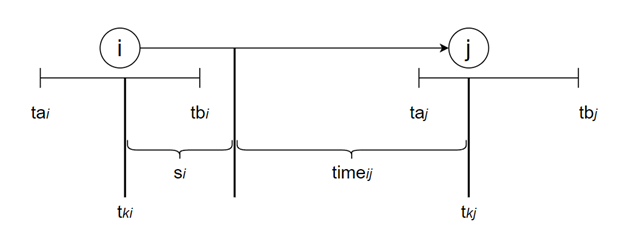
\includegraphics[width=\textwidth]{Anh/relationship_of_time_and_parameter}
		\caption{Mối quan hệ của thời gian và tham số}
		\label{relationship_of_time_and_parameter}
	\end{figure}
	\item $y_{ik}$: Khối lượng hàng trên xe sau khi đến và phục vụ điểm $i (i \in N, k\in V)$
	\begin{figure}[H]
		\centering
		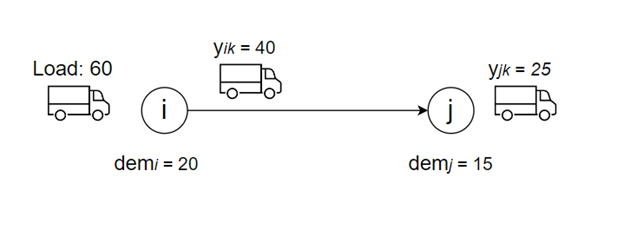
\includegraphics[width=\textwidth]{Anh/relationship_of_y_and_others_parameter}
		\caption{Mối quan hệ của y và tham số}
		\label{relationship_of_y_and_others_parameter}
	\end{figure}
\end{itemize}
\subsubsection*{Hàm mục tiêu}
\begin{align}
	\text{Minimize:} & \tong{k\in V}\tong{i\in N}\tong{j\in N} x_{ijk}.time_{ij} && \label{obj_func}\\
	\text{s.t:} & \tong{j\in N} x_{0jk} = 1 &&,\forall\, k\in V\label{cons:1}\\
	& \tong{i\in N}x_{i,n+1,k} = 1 &&,\forall\, k \in V\label{cons:2}\\
	& \tong{k\in V}\tong{j\in N} x_{ijk} = 1 &&,\forall\, i\in C\label{cons:3}\\
	& \tong{i\in N} x_{iak} - \tong{j\in N} x_{ajk} = 0 &&,\forall\, a\in C, \forall\, k\in V\label{cons:4}\\
	& \tong{i\in C} dem_i \tong{j\in N} x_{ijk} \le Q &&,\forall\, k\in V\label{cons:5}\\
	& 0 \le y_{ik} \le Q &&,\forall\, i\in C, \forall\, k \in V\label{cons:6}\\
	& y_{ik} - dem_jx_{ijk} - y_{ik} \ge T\ngoacto{x_{ijk} - 1} &&,\forall\, i, j \in N, k\in V\label{cons:7}\\
	& ta_i \le t_{ik} \le tb_i &&,\forall\, i \in N, k \in V\label{cons:8}\\
	& t_{ik} + time_{ij} + s_i - t_{jk} \le T\ngoacto{1-x_{ijk}} &&,\forall\, i, j \in N, \forall\, k \in V\label{cons:9}\\
	& x_{ijk} \in \taphop{0, 1} &&,\forall\, i, j\in N, \forall\, k\in V\label{cons:10}\\
	& t_{ik} \ge 0 &&,\forall\, i\in C, \forall\, k\in V\label{cons:11}
\end{align}
\begin{itemize}
	\item Hàm mục tiêu \ref{obj_func} cho thấy ta sẽ tìm ra chi phí ít nhất của tất cả các quãng đường đi. Ở đây ta xem khoảng cách di chuyển giữa 2 điểm tuyến tính với thời gian di chuyển
	\item Ràng buộc \ref{cons:1} và \ref{cons:2} đảm bảo rằng rất cả các xe đều xuất phát từ kho (điểm 0) và quay trở lại kho (điểm $n+1$). Nếu $x_{0, n+1, k} = 1$, có nghĩa là xe $k$ không cần sử dụng
	\item Ràng buộc \ref{cons:3}: Ràng buộc này đảm bảo rằng tất cả khách hàng đều được đi qua và mỗi xe đi qua các điểm đúng 1 lần
	\item Ràng buộc \ref{cons:4}: Ràng buộc này là phương trình cho thấy sự liên tục của 1 tuyến đường được thực hiện bởi 1 xe: Nếu xe đó đến điểm $i$ thì nó bắt buộc phải rời $i$. Trong phương trình này, ta thấy mỗi điểm trung gian $a$ trên tuyến đường của xe $k$, số đường đi từ một điểm tới $a$ bằng số đường đi từ $a$ tới điểm khác
	\item Ràng buộc \ref{cons:5}: Ràng buộc này đảm bảo rằng tổng hàng trên xe không vượt quá sức chứa của xe
	\item Ràng buộc \ref{cons:6}: Ràng buộc cho biến $y$ là tải trọng trên xe
	\item Ràng buộc \ref{cons:7}: Ràng buộc xác định mới quan hệ giữa $y$ và biến $x$
		\begin{itemize}
			\item Nếu không có tuyến đường trực tiếp từ $i$ đến $j$ bằng xe $k$, ràng buộc luôn đúng do $T = \infty$
			\item Nếu có tuyến đường trực tiếp từ $i$ đến $j$ bằng xe $k$, tải trong trên xe khi phục vụ điểm $j$ luôn nhỏ hơn hoặc bằng tải trên xe sau khi phục vụ xong điểm $i$
			\item Ràng buộc này đảm bảo không có vòng lặp xảy ra trong quá trình giao hàng như: $0\rightarrow 1 \rightarrow 2\rightarrow 1$ do sau khi phục vụ một điểm, tải trọng trên xe phải luôn giảm và lớn hơn những điểm phục vụ sau.
		\end{itemize}
	\item Ràng buộc \ref{cons:8}: Ràng buộc miền giá trị biến $t$, thời điểm xe $k$ phục vụ điểm $i$ luôn nhỏ hơn hoặc bằng thời gian đóng của điểm thứ $i$
	\item Ràng buộc \ref{cons:9}: Tương tự như ràng buộc \ref{cons:7}, đây là ràng buộc xác định mối quan hệ giữa biến $x$ và biến $t$
	\begin{itemize}
		\item Nếu không có tuyến đường trực tiếp từ $i$ đến $j$ bằng xe $k$, ràng buộc luôn đúng do $T = \infty$
		\item Nếu không tuyến đường trực tiếp từ $i$ đến $j$, thời điểm sau khi từ điểm $i$ đến điểm $j$ luôn phải nhỏ hơn hoặc bằng thời gian đóng cửa của điểm $j$
	\end{itemize}
	\item Ràng buộc \ref{cons:10}: Ràng buộc giá trị của $x$. $x$ là biến nhị phân chỉ nhận giá trị $0$ hoặc $1$
	\item Ràng buộc \ref{cons:11}: Ràng buộc giá trị của biến $t$
\end{itemize}
\newpage\section{Heuristic: Hill climbing}
\subsection{Khái quát}
Trong khoa học máy tính, \kniem{tìm kiếm cục bộ - local search} là một phương pháp heuristic để giải quyết các bài toán tối ưu tổ hợp. Tìm kiếm cục bộ có thể sử dụng trong các bài toán mà có thể được tính bằng cách tìm một giải pháp tối đa hóa một tiêu chí nào đó trong số các giải pháp được đưa ra. \\[5pt]
Ý tưởng chính của tìm kiếm cục bộ: Thay vì tìm kiếm một cách có hệ thống trong không gian tìm kiếm, chúng ta chuyển từ giải pháp này đến giải pháp lân cận bằng cách áp dụng những thay đổi nhỏ cục bộ đến khi một giải pháp có thể được coi là tối ưu tổ hợp đạt được. \\
Những bài toán VRP đã được chứng minh là lớp bài toán NP khó. Vì vậy để giải quyết những bài toán thuộc họ VRP, chúng ta sẽ cố gắng tìm ra được giải pháp tối ưu nhất trong phạm vi. Để giải quyết vấn đề VRPTW, chúng ta sẽ cùng tìm hiểu một thuật toán cục bộ: \kniem{thuật toán leo đồi - Hill Climbing}.
\subsection{Cơ sở lý thuyết}
\subsubsection{Ý tưởng thuật toán}
Thuật toán leo đồi là một thuật toán tìm kiếm cục bộ (local search)
\begin{itemize}
	\item Thuật toán lấy ý tưởng từ việc "leo đồi" vì nó hoạt động theo hướng đi lên sườn đồi theo giá trị của hàm mục tiêu
	\item Một giải pháp trong không gian tìm kiếm được gọi là trạng thái. Trạng thái được biểu diễn với một vector các biến quyết định
	\item Các trạng thái sẽ được đánh giá bởi hàm mục tiêu. Lân cận của một trạng thái được xác định bằng cách thay đổi các biến quyết định của trạng thái đó.
\end{itemize}
\begin{thuattoan}
	Thuật toán Hill Climbing Search thực hiện việc di chuyển từ một trạng thái $S$ đến trạng thái $S'$ mới trong một cấu trúc lân cận xác định theo các bước sau: 
	\begin{itemize}
		\item \textbf{Bước 1: } Khởi tạo trạng thái $S$ ban đầu. Bước này có thể thực hiện bằng cách sinh ngẫu nhiên hoặc sử dụng thuật toán tham lam, heuristic khác. Tính giá trị của hàm mục tiêu $f(S)$
		\item \textbf{Bước 2: } Sinh tập lân cận $N(S')$. Tìm ra trạng thái $S'$ sao cho giá trị hàm mục tiêu $f(S')$ là bé nhất trong tất cả các lân cận
		\item \textbf{Bước 3: } Kiểm tra xem có chấp nhận di chuyển từ $S$ sang $S'$ bằng cách so sánh hàm mục tiêu. Nếu chấp nhận thì thay $S$ bằng $S'$, nếu không có thì giữ nguyên trạng thái $S$
		\item \textbf{Bước 4: } Kiểm tra điều kiện dừng, điều kiện dừng có thể là số vòng lặp hoặc khi giá trị hàm mục tiêu không thay đổi qua nhiều bước lặp
	\end{itemize}
\end{thuattoan}
\subsubsection{Một số vấn đề của thuật toán leo đồi }
\begin{figure}[H]
	\centering
	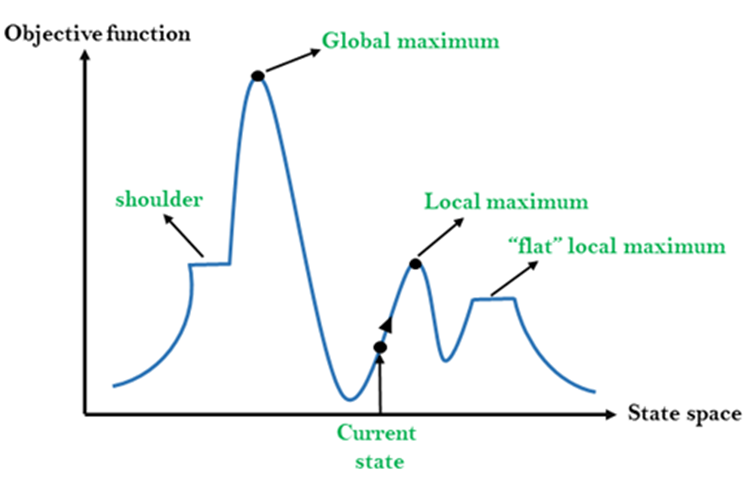
\includegraphics[width=0.9\textwidth]{Anh/mo_ta_leo_doi}
	\caption{Vấn đề của thuật toán leo đồi}
\end{figure}
\begin{itemize}
	\item Bẫy tối ưu cục bộ: Đây là vấn đề lớn nhất của thuật toán Hill Climbing. Thuật toán có thể rơi vào một điểm tối ưu cục bộ, đó là khi nó đã leo lên đến một đỉnh và các lân cận đều cho giá trị hàm mục tiêu nhỏ hơn nhưng đỉnh này có thể chưa phải là đỉnh cao nhất. Như vậy hiệu quả của thuật toán phụ thuộc rất nhiều vào trạng thái ban đầu cũng như bề mặt của không gian tìm kiếm.
	\item Cao nguyên (Shoulder): Cao nguyên  là khi không gian tìm kiếm của trạng thái bằng phẳng, có nghĩa là giá trị hàm mục tiêu của các lân cận, lân cận của lân cận đều bằng nhau. Trong trường hợp đó, chúng ta không thể xác định được hướng đi để có thể thoát khỏi cao nguyên.
\end{itemize}
\subsection{Phương pháp thực hiện}
Để áp dụng thuật toán leo đồi để giải bài toán VRPTW, chúng ta cần giải quyết các vấn đề như: Thiết lập lời giải ban đầu, sinh ra được tập lân cận của $S$, thiết lập hàm mục tiêu đánh giá lời giải, điều kiện dừng. Sau đây ta sẽ phân tích từng vấn đề.
\subsubsection{Tạo lời giải ban đầu}
Lời giải ban đầu có thể tạo bằng cách sinh ngẫu nhiên từng điểm rồi đưa chúng vào các tuyến đường sao cho đảm bảo các ràng buộc về thời gian và khối lượng. Tuy nhiên như đã phân tích ở phần 6.2.2, thuật toán phụ thuộc nhiều vào trạng thái ban đầu do có thể rơi vào điểm tối ưu cục bộ. Vì vậy sinh ngẫy nhiên không phải là giải pháp tốt.\\
\paragraph*{Thuật toán tham lam để tạo ra lời giải ban đầu:} Ý tưởng của thuật toán tham lam là ta sẽ tạo ra các tuyến xe phục vụ các điểm theo từng cụm, như vậy chi phí quãng đường đi sẽ có thể được đảm bảo  hơn việc sinh ngẫu nhiên.
\begin{thuattoan}[Thuật toán tham lam] .
	\begin{itemize}
		\item Cấu trúc dữ liệu:
		\begin{itemize}
			\item List các khách hàng
			\item List các tuyến xe, mỗi phần tử của dãy là một vector các khách hàng
			\item List ứng cử viên
		\end{itemize}
		\item Sắp xếp các khách hàng qua một trọng số "độ phân cụm về vị trí và thời gian" của các khách hàng
		\item Duyệt khách hàng $i$ trong danh sách các khách hàng đã được sắp xếp:
		\begin{itemize}
			\item Duyệt qua tất cả các tuyến xe $V$ hiện có:
			\begin{itemize}
				\item Duyệt khách hàng $j$ đang tồn tại trong tuyến xe $V$
				\item Chèn khách hàng $i$ trước khách hàng $j$. Nếu trạng thái sau khi chèn thỏa mãn tất cả các ràng buộc về thời gian, khối lượng, ta đưa nó vào list ứng cử viên
				\item Xóa khách hàng $i$ khỏi tuyến xe $V$
			\end{itemize}
			\item Nếu tập ứng cử viên trống, ta tạo ra một tuyến xe mới và đưa khách hàng $i$ vào tuyến đó.
			\item Nếu tập ứng cử viên không trống, chọn ra ứng cử viên với tổng khoảng cách di chuyển của tất cả các xe là ít nhất. Ta chọn ứng cử viên đó gán cho khách hàng $i$
		\end{itemize}
	\end{itemize}
\end{thuattoan}
\paragraph*{Phân tích về các cách sắp xếp khách hàng với trọng số "độ phân cụm"}.\\
Ta gọi góc lượng giác $\alpha\in\doan{-\pi}{\pi}$ là \kniem{độ lệch} giữa kho (depot) và khách hàng trong mặt phẳng tọa độ $Oxy$
\begin{figure}[H]
	\centering
	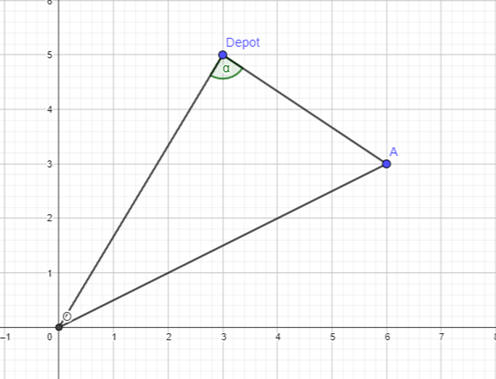
\includegraphics[width=0.6\textwidth]{Anh/minhhoa_thamlam}
	\caption{Mô tả độ lệch $\alpha$}
\end{figure}
\begin{itemize}
	\item Nếu lấy $O$ là gốc tọa độ, $D$ là kho và $A$ là khách hàng thì $\alpha = \angle\ngoacto{DO, DA}$.
	\item Nếu kho chính là gốc tọa độ thì $\alpha = \angle\ngoacto{Ox, OA}$.
\end{itemize}
Cách tính góc $\alpha$:\\
Ta có:
\begin{align*}
    &\dfrac{OA}{\sin\alpha} = \dfrac{AD}{\sin DOA}&\quad\text{(theo định lý $\sin$)}\\
    \Rightarrow& \sin\alpha = \dfrac{\sin DOA. OA}{AD}&\\
    \Leftrightarrow& \alpha = \arcsin\ngoacto{\dfrac{\sin DOA. OA}{AD}}&\\
\end{align*}
Lại có: $$\angle DOA = \angle DOx - \angle AOx= \arctan\dfrac{y_D}{x_D}-\arctan\dfrac{y_A}{x_A}$$


% chỗ này có công thức toán học chưa viết xong

Thuật toán thực hiện tham lam ở hai bước: 
\begin{itemize}
	\item Một là sắp xếp khách hàng theo trọng số là góc $\alpha$.
	\item Hai là với tập ứng cử viên, ta luôn chọn ứng cử viên để tổng khoảng cách các xe ở thời điểm xét đến khách hàng hiện tại là bé nhất. Tuy nhiên, nếu ta chọn ứng cử viên khác thì có thể trong tương lai sẽ thu được một giải pháp tốt hơn.
\end{itemize}
\subsubsection{Tìm kiếm các lân cận của trạng thái hiện tại}
Với thuật toán leo đồi, tại mỗi bước lặp sẽ có quá trình sinh ra các trạng thái lân cận, so sánh chất lượng của trạng thái đó với các trạng thái lân cận. Việc xác định được các lân cận chất lượng cũng là yếu tố để bài toán có thể đạt được giá trị tối ưu. Trong phần này, ta sẽ đưa ra 4 phương pháp tìm kiếm lân cận phổ biến trong ngữ cảnh của các bài toán VRP:
\begin{pphap}[Relocate method]
	Phương pháp này là việc di chuyển một khách hàng sang tuyến đường khác. Khách hàng $i$ sẽ bị xóa đi khỏi tuyến đường $r_0$ và chuyển sang vị trí mới của tuyến đường $r_1$
\end{pphap}
\begin{vd}
	Từ hình \ref{relocate_method} Khách hàng $5$ ở tuyến đường $1$ sẽ được chuyển sang vị trí $4$ của tuyến $2$
\begin{figure}[H]
	\centering
	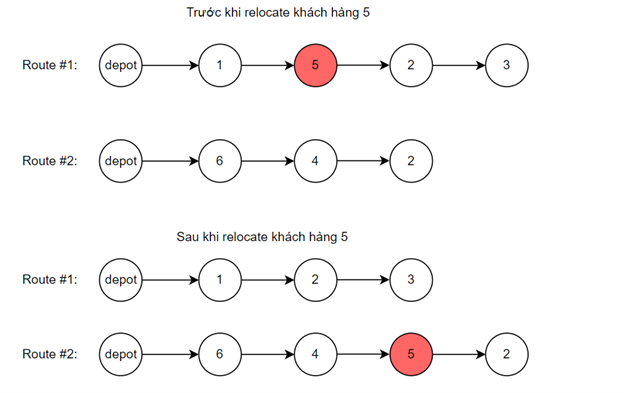
\includegraphics[width=0.9\textwidth]{Anh/relocate_method}
	\caption{Minh họa relocate method}
	\label{relocate_method}
\end{figure}
\end{vd}
\paragraph{Phương pháp thực hiện}: Random ngẫu nhiên khách hàng $c_i$ ở tuyến đường ngẫu nhiên $r$. Thực hiện relocate cho khách hàng đó với tất cả các tuyến đường. Nếu trạng thái relocate thỏa mãn ràng buộc, đưa vào danh sách ứng cử viên. Chọn ra ứng cử viên tốt nhất:
\begin{thuattoan}
	.
	\begin{itemize}
		\item $R$ = random in route
		\item $C$ = random in $R$
		\item For each route in routes
		\item For each position in route.nodes
		\begin{itemize}
			\item Relocate(C, position, route)
			\item if (check(route) == True) then candidates.push(C, position, route)
		\end{itemize}
		\item Min\_candidate = min (values(candidate) in candidates)
	\end{itemize}
\end{thuattoan}
\begin{pphap}[Swap method]
	Phương pháp này đổi chỗ hai vị trí trên cùng một tuyến đường
\end{pphap}
\begin{vd}
	Trong cùng một tuyến đường, khách hàng $c_i$ ở vị trí $p_i$ sẽ đổi chỗ với khách hàng $c_j$ ở vị trí $p_j$ (hình \ref{swap_method})
\begin{figure}[H]
	\centering
	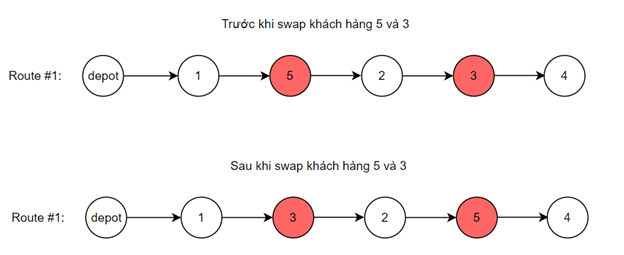
\includegraphics[width=0.9\textwidth]{Anh/swap_method}
	\caption{Minh họa swap method}
	\label{swap_method}
\end{figure}
\end{vd}
\paragraph{Phương pháp thực hiện}: Random ngẫu nhiên một khách hàng. Thực hiện swap tất cả các khách hàng trong tuyến đường đó. Nếu trạng thái swap thỏa mãn ràng buộc, đưa vào danh sách ứng cử viên. Chọn ra ứng cử viên tốt nhất
\begin{thuattoan}
	.
	\begin{itemize}
		\item $R$ = random in route
		\item For each position1 in R.nodes
		\item For each position2 in R.nodes
		\begin{itemize}
			\item Swap(position1, position2)
			\item If (check(R) == True) then candidates.push(position1, position2)
		\end{itemize}
		\item Min\_candidate = Min(values(candidate) in candidates)
		\item Swap(min\_candidate)
	\end{itemize}
\end{thuattoan}
\begin{pphap}[Cross exchange]
	Đối với phương pháp này, hai khách hàng ở hai tuyến đường khác nhau sẽ đổi bị trí cho nhau. Phương pháp này có thể xem như sử dụng hai lần relocate với hai khách hàng
\end{pphap}
Cụ thể hơn, khách hàng $c_i$ đang ở vị trí $p_i$ ở tuyến đường $r_1$ sẽ đổi chỗ cho khách hàng $c_j$ ở vị trí $p_j$ của tuyến đường $r_2$ (hình \ref{cross_exchange})
\begin{figure}[H]
	\centering
	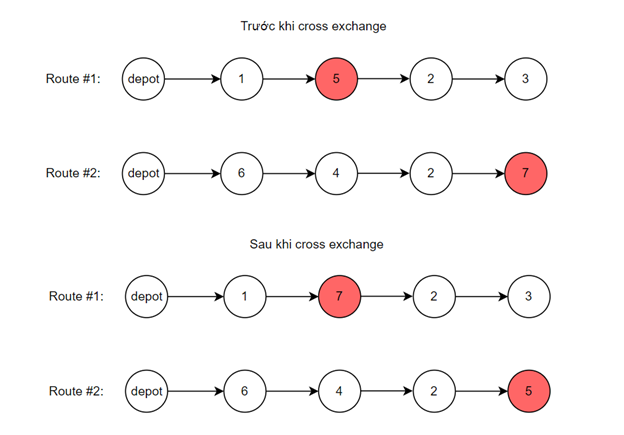
\includegraphics[width=0.9\textwidth]{Anh/cross_exchange}
	\caption{Minh họa cross exchange}
	\label{cross_exchange}
\end{figure}
\paragraph{Phương pháp thực hiện}: Random ngẫu nhiên một khách hàng $c_i$ ở tuyến đường ngẫu nhiên $r$. Thực hiện exchange cho khách hàng đó với tất cả các khách hàng khác. Nếu trạng thái exchange thỏa mãn ràng buộc, đưa vào danh sách ứng cử viên. Chọn ra ứng cử viên tốt nhất
\begin{thuattoan}
	.
	\begin{itemize}
		\item $R$ = random in route
		\item $C$ = random in $R$
		\item For each route in routes
		\item For each position in route.nodes
		\begin{itemize}
			\item CrossExchange(C, position, route)
			\item If (check(route) == True) then candidates.push(C, position, route)
		\end{itemize}
		\item Min\_candidate = Min(values(candidate) in candidates)
	\end{itemize}
\end{thuattoan}
\begin{pphap}[Move method]
	Phương pháp này sẽ tách một khách hàng và đưa nó ra một tuyến đường mới.
\end{pphap}
Khách hàng $c_i$ ở tuyến đường $r$ sẽ được tách thành một tuyến đường mới (Hình \ref{move_method})
\begin{figure}[H]
	\centering
	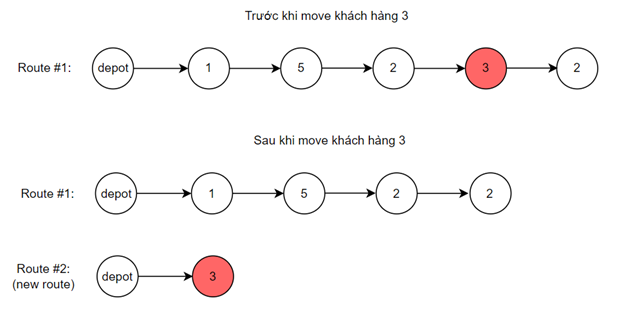
\includegraphics[width=0.9\textwidth]{Anh/move_method}
	\caption{Minh họa move method}
	\label{move_method}
\end{figure}
\paragraph{Phương pháp thực hiện} Random ngẫu nhiên một tuyến đường. Thực hiện move tất cả các khách hàng trong tuyến đường và đưa vào danh sách ứng cử viên. Chọn ra ứng cử viên tốt nhất.
\begin{thuattoan}
	.
	\begin{itemize}
		\item $R$ in route
		\item For each position in R.nodes
		\begin{itemize}
			\item Move(position)
			\item candidates.push(position)
		\end{itemize}
		\item Min\_candidate = Min(values(candidate) in candidates)
	\end{itemize}
\end{thuattoan}
\subsubsection{Điều kiện dừng}
Đối với bài toán, điều kiện dừng là khi vòng lặp chạy đủ 10000 lần
\begin{thuattoan}[Tổng quát thuật toán leo đồi với bài toán VRPTW]
	Procedure HillClimbing:
	\begin{itemize}
		\item Current = generate solution by greedy method
  \item max\_iter = 10000
		\item Loop do:
		\begin{itemize}
			\item neighbor = min value in local of current
			\item if (Value(neighbor) < Value(current)) then current = neighbor
                \item if iter > max\_iter then break
                \item iter = iter + 1
		\end{itemize}
	\end{itemize}
\end{thuattoan}
\subsection{Kết quả thực hiện}
Với bộ test solomon, đây là kết quả thực hiện được
\begin{longtblr}[
	caption = {Kết quả thực hiện Hill-climbing},
	label = {tab:test},
	]{
		colspec = {|X[c,m]|X[c,m]|X[c,m]|X[c,m]|X[c,m]|},
		rowhead = 1,
		hlines,
		row{even} = {gray9},
		row{1} = {olive9},
	} 
	Testcase Name	& Number of Vehicles	& Total Distance	& Optimal Solution	& Execution Time \\
	C101&	11&	827.3&	827.3&	1.61 \\
	C102&	11&	892.8&	827.3&	1.92\\
	C103&	12&	1077&	826.3&	2.29\\
	C104&	12&	958.1&	822.9&	2.67\\
	C105&	11&	874.5&	827.3&	1.66\\
	C106&	11&	827.3&	827.3&	1.89\\
	C107&	11&	827.3&	827.3&	1.97\\
	C108&	11&	827.3&	827.3&	2.12\\
	C109&	11&	902.1&	827.3&	2.21\\
	C201&	4&	621.2&	589.1&	2.41\\
	C202&	4&	634.1&	588.7&	4.02\\
	C204&	5&	709.5&	588.1&	5.1\\
	C205&	4&	586.4&	586.4&	3.2\\
	C206&	4&	586&	586&	3.6\\
	C207&	5&	618.4&	585.8&	3.85\\
	C208&	4&	585.8&	585.8&	3.83\\
	R101&	24&	1641.4&	1637.7&	1.84\\
	R102&	18&	1405.4&	1466.6&	2.01\\
	R103&	14&	1210.5&	1208.7&	1.88\\
	R104&	13&	1068.6&	971.5&	2.46\\
	R105&	18&	1464.4&	1355.3&	1.85\\
	R106&	15&	1269.8&	1234.6&	1.97\\
	R107&	14&	1202.5&	1064.6&	2.31\\
	R108&	13&	1117.7&	932.1&	2.39\\
	R109&	16&	1280.7&	1146.9&	1.94\\
	R110&	16&	1234.4&	1068&	2.03\\
	R111&	14&	1198&	1048.7&	2.1\\
	R112&	14&	1113.9&	948.6&	2.2\\
	R201&	6&	1392.2&	1143.2&	2.2\\
	R202&	6&	1227.3&	1029.6&	2.78\\
	R203&	5&	1061.3&	870.8&	3.39\\
	R204&	4&	944.7&	731.3&	4.61\\
	R205&	5&	1187.2&	949.8&	3.08\\
	R206&	4&	1101.8&	875.9&	2.71\\
	R207&	4&	1083.9&	794&	6.52\\
	R208&	4&	822.4&	701&	5.63\\
	R209&	5&	1118.8&	854.8&	2.84\\
	R210&	6&	1078.7&	900.5&	3.7\\
	R211&	4&	975.7&	746.7&	5.21\\
	RC101&	19&	1723.7&	1619.8&	1.84\\
	RC102&	17&	1541.6&	1457.4&	1.89\\
	RC103&	14&	1357.5&	1258&	2.02\\
	RC104&	14&	1306&	1132.3&	2.52\\
	RC105&	18&	1562.7&	1513.7&	1.91\\
	RC106&	16&	1424.1&	1372.7&	1.94\\
	RC107&	14&	1255.9&	1114.2&	2.22\\
	RC201&	8&	1498.2&	1261.8&	2.26\\
	RC202&	5&	1359.4&	1092.3&	2.19\\
	RC203&	4&	1130&	923.7&	2.78\\
	RC204&	5&	983&	783.5&	5.04\\
	RC205&	7&	1459.7&	1154&	2.27\\
	RC206&	7&	1325.1&	1051.1&	2.36\\
	RC207&	7&	1239.7&	962.9&	3.29\\
	RC208&	5&	1084&	776.1&	4.35\\
\end{longtblr}
\begin{nx}
	Ta thấy:
	\begin{itemize}
		\item Với những bộ test C là những test phần cụm thì kết quả cho ra khá tốt. Có nhiều test đạt được kết quả tối ưu.
		\item Với những bộ test R là random ngẫu nhiên các khách hàng thì kết quả cho ra xấp xỉ 80\% kết quả tối ưu. Tương tự với những test RC.
		\item Tuy vậy vẫn còn một số test C cho ra kết quả khá tệ như test C103 với kết quả tìm được là 1077 so với kết quả tối ưu 826,3. Điều này rất có thể do thuật toán đã đi vào bẫy tối ưu cục bộ hoặc đi vào một cao nguyên nào đó. 
		\item Với thời gian chạy trung bình là 2,81 s, thuật toán hoàn toàn có thể chạy được với những test $n = 100$. Tuy nhiên trong những bộ thực tế thì $n$ có thể lớn hơn rất nhiều vì vậy có thể giảm số vòng lặp của điều kiện dừng để đảm bảo thời gian chạy. Tuy nhiên khi đó chất lượng của lời giải chắc chắn sẽ bị giảm đi. 
	\end{itemize}
\end{nx}
\section{Tổng kết}
Báo cáo đã đưa ra 4 thuật toán, tương ứng với đó là 3 phương pháp để giải quyết bài toán VRPTW. Đối với những thuật toán chính xác, đầu tiên là phương pháp vét cạn toàn bộ trường hợp, sau đó xây dựng mô hình QHTT với thuật toán giải quyết bài toán QHTT, quy hoạch nguyên. Tiếp đó là phương pháp heuristic tìm kiếm cục bộ với thuật toán tìm kiếm leo đồi. Với phương pháp đó đã giải quyết được các bài toán với số lượng $n$ lớn. Tuy vậy chất lượng lời giải vẫn chưa đảm bảo do tính hạn chế của thuật toán. Để cải thiện chất lượng lời giải, chúng ta có thể sử dụng những thuật toán meta heuristic, thuật toán tiến hóa như Tabu Search, thuật toán di truyền, \ldots. Tuy nhiên vì thời gian hạn chế, nhóm đã không thể tìm hiểu cũng như cài đặt các thuật toán đó. Trong tương lai, chúng em sẽ cố gắng phát triển các thuật toán nâng cao hơn, để đồ án có tính đóng gói hoàn thiện đúng theo chiều dài lịch sử của vấn đề. \\ [5pt]
Cuối cùng, nhóm chúng em xin cảm ơn thầy Nguyễn Khanh Văn đã góp ý, hỗ trợ chúng em trong quá trình thực hiện project 1. Do bản thân có ít kinh nghiệm kỹ năng, báo cáo khó tránh khỏi các thiếu sót. Em rất mong nhận được sự chỉ bảo, góp ý của thầy để bản thân ngày càng hoàn thiện hơn.
\newpage\section{Tài liệu tham khảo}
\begin{thebibliography}{9}
\bibitem{lttu}
Nguyễn Thị Bạch Kim, Giáo trình Các Phương Pháp Tối Ưu Lý Thuyết Và Thuật Toán, Nhà xuất bản đại học Bách khoa, Hà Nội, 2006. 
\bibitem{lamport94}
Bùi Thế Tâm, Quy hoạch rời rạc, Nhà xuất bản đại học sư phạm, Hà Nội, 2008.
\bibitem{vhc}
Vehicle Routing Problems, Methods and Applications (Second Edition), Paolo Toth, Danielo Vigo, 2002.
\bibitem{rtp}
Local search for the vehicle routing problem, Yves Deville, 2015. 
\end{thebibliography}
\section{Phụ lục}
\large Link mã nguồn : \href{https://github.com/Dangptpt/VRPTW}{https://github.com/Dangptpt/VRPTW}
\end{document}              
